\setchapterstyle{kao}
\setchapterpreamble[u]{\margintoc}
\chapter{Digital interfaces for environmental sensors}
\labch{digital_interfaces}

In \refch{circuits_intro}, we considered the fundamentals of constructing circuits that exploit the abilities of microcontrollers to measure voltage and time to quantify environmental variables.
These circuits were based on \textit{analog} sensors -- that is, sensors that return signals in the form of continuously variable voltages or time lags.
By integrating the microcontroller, circuit and analog sensor components, you assembled a device that provided a \textit{digital} signal -- a number that represents an observation of the corresponding environmental parameter.

A modern trend in sensor development is \textit{digital sensors}, whose output is intrinsically in the form of numbers rather than voltage or time.
If you used the external \DS3231 Real Time Clock in \refch{time_keeping}, you have already used a digital sensor.
In digital sensors, the circuitry and some of the microcontroller functions that you used to convert analog signals to digital outputs have been placed on the sensor itself.
This means that the user-designed circuitry and microcontroller interfaces can usually be greatly simplified compared to an analog sensor measuring the same quantity.

Because digital sensors typically return observations as numbers with many decimal places, it's tempting to overlook the fact that in many cases they may be less accurate and precise than analog sensors (or may cost more for comparable accuracy and precision).
It's important to keep in mind that digital sensors have the same basic operating principles and limitations as analog sensors.
The internal circuitry of digital sensors is designed by experts and mass-produced in sophisticated factories.
This means that the tradeoffs and optimizations in sensitivity, resolution, power consumption, \etc that you considered in working with analog sensors have been decided by highly skilled professionals.
Remember, though, that these circuits (and hence the digital sensors that use them) still have most of the same constraints you wrestled with in your own sensor design.

With those caveats in mind, digital sensors often have a number of advantages relative to analog sensors.
Depending on the type of digital sensor and the context, these advantages may include:
\begin{itemize}
	\item Digital sensors use digital \texttt{GPIO}s, which are more abundant than analog \texttt{GPIO}s on most microcontrollers;
	\item Protocols for communicating with digital sensors are two-way -- information such as settings, commands to take readings \etc can be sent to digital sensors to make them more efficient and versatile;
	\item Some digital sensor protocols support multiple sensors on one set of \texttt{GPIO}s and wires, with microcontrollers able to identify and query each of those sensors individually;
	\item Some digital protocols support very long wire connections (though others are limited to very short wires);
	\item Some digital sensors internally do complex computations, such as integrating angular orientation from angular accelerations, which would be expensive in terms of processor cycles and energy to perform on a microcontroller.
\end{itemize}
These advantages are evident in many industrial applications (cars, phones, \etc).
As a result, many useful digital environmental sensors are mass produced and amazingly cheap for their capabilities.

This chapter uses examples of readily available and scientifically informative environmental sensors to illustrate how to use several common communication protocols for digital sensors.
Many other examples using each of these protocols appear later in this book, in applications of data from digital sensors to drawing inferences and hypothesis testing about environmental mechanisms.
For some readers, one or two of these protocols may be sufficient for the examples and data collection applications at hand.
If so, it may be an efficient strategy to focus on that subset of protocols, returning to learn the others if and when the need arises.

\subsection{Communicating with digital sensors}
In practice, getting measurements from digital sensors usually involves two main elements: establishing the appropriate circuit connections, and finding (or, occasionally, writing) a \emph{driver}.
A driver is a piece of code that interfaces between a microcontroller and digital sensor.
The driver enables the user to interact with a digital sensor, \eg by setting measurement parameters or querying for data, with simple, intuitive high-level \Micropython commands.
The driver handles messages between the microcontroller and the digital sensor at a very low level, that takes some technical expertise and patience to understand.
Fortunately, \Micropython-based drivers are freely available online for many of the most useful digital environmental sensors, and more are being written all the time.
You typically don't need to know much about the inner workings of a driver to use it for obtaining environmental sensor readings.

Most digital sensors used in environmental sensing communicate using one of four protocols:

%\begin{itemize}
%	\item \textbf{Inter-Integrated Circuit (\i2c)}
%
%	The \htmladdnormallink{\i2c}{https://en.wikipedia.org/wiki/I\%C2\%B2C} protocol (pronounced ``eye squared sea'') is commonly used in digital sensors for time, light, accceleration, \etc, and is also used in many small TFT displays for microcontrollers.
%	%Adafruit provides a useful \htmladdnormallink{overview of \i2c}{https://learn.adafruit.com/adafruit-ft232h-with-spi-and-i2c-libraries/i2c-devices}.
%	\i2c is a ``2 wire'' protocol (in addition to \texttt{Vin} and \texttt{GND}).
%	\i2c is designed to work over relatively short distances ($\le$ a few meters), but \htmladdnormallink{\texttt{differential extenders}}{https://learn.sparkfun.com/tutorials/qwiic-differential-i2c-bus-extender-pca9615-hookup-guide/all} are available that greatly increase the distance over which \i2c devices can communicate.
%
%	\smallskip
%	\i2c supports multiple devices on one cable, but each device must have unique addresses.
%	Adafruit has written a useful \htmladdnormallink{summary of default \i2c addresses}{https://cdn-learn.adafruit.com/downloads/pdf/i2c-addresses.pdf}, describing addresses used by different types of sensors and other devices.
%	Because there are more types of devices than distinct addresses, there is overlap between the addresses of some different sensor types.
%	It's largely a matter of luck whether two sensor types have conflicting addresses, but works out most of the time.
%	Some \i2c devices have a mechanism, like movable jumpers, to change \i2c addresses so that two or more of these devices can co-exist on the same cable.
%
%	\item \textbf{1-Wire}
%
%	\htmladdnormallink{1-wire}{https://en.wikipedia.org/wiki/1-Wire} is a proprietary protocol design that, as the name implies, uses only one wire in addition to \texttt{Vin} and \texttt{GND}.
%	1-wire is used in relatively few sensor types, but is worth knowing about because one of those is an inexpensive and versatile \htmladdnormallink{temperature sensor}{https://datasheets.maximintegrated.com/en/ds/DS18B20.pdf} that is among the most useful available for environmental monitoring.
%
%	\smallskip
%	1-wire supports many (up to hundreds) of devices on a single cable, each of which can be independently queried for sensor readings because it has a unique ROM address.
%	1-wire supports lower (but still generally sufficient) data rates than \i2c, which (when properly configured) can operate over much longer cables.
%
%	\item \textbf{Universal Asynchronous Receiver-Transmitter (\uart)}
%
%	\htmladdnormallink{\uart}{https://en.wikipedia.org/wiki/Universal_asynchronous_receiver-transmitter} is a communications protocol with a long history of use in computer hardware (including communication between computers and microcontrollers), navigation equipment and many other industrial applications.
%	\uart supports communication between only two devices, and these devices must share common settings for a number of parameters. %(bit speed, character length, parity, and stop bits).
%	Common applications in environmental sensing include \texttt{GPS} receivers and Air Quality Index sensors.
%
%	\uart uses two wires (in addition to \texttt{Vin} and \texttt{GND}), one for transmitting and one for receiving.
%	In some applications (\eg, some \texttt{GPS} configurations) only one of these functions is utilized (\eg, transmit on the \texttt{GPS} and receive on the microcontroller) in which case only one of these wires is necessary.
%
%	\item \textbf{Serial Peripheral Interface (\spi)}
%
%	The \spi protocol is commonly used for some types of sensors, external radio communications, TFT displays, LED banks, \etc
%	\spi uses four wires (in addition to \texttt{Vin} and \texttt{GND}), three of which can be shared by multiple devices on the same cable but the fourth of which must be unique to each device.
%	Maximum data rates are higher than for \i2c devices.
%	Many digital sensors have both \spi and \i2c interfaces, so they can be used with either protocol.
%
%	%►Overview: https://learn.sparkfun.com/tutorials/serial-peripheral-interface-spi
%	%Technical info: https://en.wikipedia.org/wiki/Serial\_Peripheral\_Interface\_Bus
%	%Also see Adafruit tutorials on SPI sensors
%\end{itemize}

\begin{itemize}
	\item \textbf{Inter-Integrated Circuit (\i2c)}

	The \htmladdnormallink{\i2c}{https://en.wikipedia.org/wiki/I\%C2\%B2C} protocol (pronounced ``eye squared sea'') is commonly used in digital sensors for time, light, accceleration, \etc, and is also used in many small TFT displays for microcontrollers.

	\item \textbf{1-Wire}

	\htmladdnormallink{1-wire}{https://en.wikipedia.org/wiki/1-Wire}  is used in relatively few sensor types, but is worth knowing about because one of those is an inexpensive and versatile \htmladdnormallink{temperature sensor}{https://datasheets.maximintegrated.com/en/ds/DS18B20.pdf} that is among the most useful available for environmental monitoring.


	\item \textbf{Universal Asynchronous Receiver-Transmitter (\uart)}

	\htmladdnormallink{\uart}{https://en.wikipedia.org/wiki/Universal_asynchronous_receiver-transmitter} is a communications protocol with a long history of use in computer hardware, including communication between computers and microcontrollers.
	\uart is used in many Global Positioning System (GPS) receivers and Air Quality Index (AQI) sensors, in some Automatic Identification System (AIS) navigation equipment, and many other industrial applications.

	\item \textbf{Serial Peripheral Interface (\spi)}

	The \htmladdnormallink{\spi}{https://learn.sparkfun.com/tutorials/serial-peripheral-interface-spi} protocol is commonly used for some types of sensors (including cameras), external radio communications, TFT displays, LED banks, \etc
	Perhaps most usefully in for applications with microcontrollers, \spi interfaces are often used to read from and write to microSD cards.
\end{itemize}

\subsection{Data types and serial communication}

To interpret digital data from a sensor, we’ll need to know a little about a few standard formats used to represent data.  
At the most basic level, all digital data consists simply of bits, that is, individual values of either 1 or 0 (specifically transistors on a microchip that are either on or off).
This type of data is referred to as binary data.

It is possible to represent any integer value using bits. Take for example the three-bit number, 110 (or, more precisely, on-on-off). There are two possible states for the right-most (or least significant) bit, two possible states for the middle bit, and two possible states for the left-most (or most significant) bit, yielding eight total bit combinations. The standard convention for computing an integer from a sequence of $n$ ordered bits (i.e., bit$_1$, bit$_{2}$, ..., bit$_n$, where $n$ represents the index of the least significant bit) is  

\begin{equation}
\label{eq:base2}
\text{\parbox[c]{1.5cm}{\raggedright Integer value}} = 2^{n-1}*\text{bit}_1 +  2^{n-2}*\text{bit}_{2} + ... + 2^0*\text{bit}_{n}
\end{equation}

For the three-bit number 110, the integer equivalent is thus 2\textsuperscript{2}*1 + 2\textsuperscript{1}*1 + 2\textsuperscript{0}*0 = 6.  

By convention, binary data is organized into packets known as bytes that are eight bits long.  In a single byte, there are a total of 2\textsuperscript{8} (or 256) possible cominations of bits.
About half of the possible combinations of bits in a byte have been assigned to specific characters or commands on a computer keyboard.
These commands are usually referred to as \texttt{ASCII} characters, or sometimes just text.
When you save data as a \texttt{.txt} file, each character you save is really just the byte of information representing the character.

Just like with \texttt{ASCII} text, each possible combination of bits in a byte corresponds to an integer value that ranges from 0 to 255.
It is possible to combine multiple bytes to represent larger numbers.  Here, for an $n$-digit number in a system where each digit represents \emph{b} possible states (we refer to \emph{b} as the \emph{base} of the number), the general formula becomes

\begin{equation}
\label{eq:base}
\text{\parbox[c]{1.5cm}{\raggedright Integer value}} = b^{n-1}*\text{digit}_1 + b^{n-2}*\text{digit}_{2} + ... + \text{digit}_{n} 
\end{equation}

In the decimal system, this is easy to understand--we all know that the base-10 decimal number 326 = 3*10\textsuperscript{2} + 2*10\textsuperscript{1} + 6.
However, it also works if each digit represents a byte (so 256 combinations, or base 256).  
For example, for two bytes in sequence, the integer equivalent can be found by multiplying the 0-255 value of the first (i.e, most significant) digit by 256 and then adding this to the value of the second (or least significant) digit.
The general formula for a 2-byte (aka 16 bit) number would thus be

\begin{equation}
\label{eq:base256}
\text{\parbox[c]{1.5cm}{\raggedright Value of two byte number}} = 256 *\text{\parbox[c]{1.5cm}{\raggedright integer value of byte 1}} + \text{\parbox[c]{1.5cm}{\raggedright integer value of byte 2}} 
\end{equation}

For example, if the integer value of the first byte in a two-byte sequence is 95 and the integer value of the second byte in the two-byte sequence is 5, the result would be 256*95 + 5, or 24320.

For low-level computer programmers who want to work with bytes regularly, there is a fourth convention for representing data that is known as the hexadecimal system.
It is extremely common to see digital numbers sent from sensors represented this way, so it is important to understand how hexadecimal numbers work.
In this system, data is thought of as being stored in chunks that are half a byte (so four bits) long.
This chunk of data is sometimes referred to as a nibble.
There are 16 possible combinations of bits in a nibble, so the integer value of a byte can be found from two nibbles in sequence as follows:

\begin{equation}
\label{eq:base16}
\text{\parbox[c]{1.5cm}{\raggedright integer value of byte}} = 16 *\text{\parbox[c]{1.5cm}{\raggedright integer value of nibble 1}} + \text{\parbox[c]{1.5cm}{\raggedright integer value of nibble 2}} 
\end{equation}

It would be awkward to write out the actual combinations of ones and zeros in each of the 16 possible bit combinations in a nibble.
Because there are only 16 possible combinations, the convention is to use the numerals 0 to 9 to represent the first 10 combinations, then to use the letters A to F to represent the remaining six combinations.
Two nibbles in sequence represents a full bit, so in the hexadecimal system, a byte can be written, for example, as 4E, with the 4 representing the bit combination 0100 and E representing the bit combination 1110.
Together, with the “E” combination written second, this actually represents the byte 01001110, the \texttt{ASCII} character capital “N,” or the decimal number 78.
Full conversions between each number system are provided in Table \ref{tab:convert}.  

If you look closely at Table \ref{tab:convert}, you’ll see that in the \texttt{ASCII} system, only 128 of the possible 256 bit combinations are actually assigned to characters or keyboard commands.
There is no single standard for representing the other 128 combinations as text.  
However, any byte can be represented using a sequence of two hexadecimal numbers.
So, if we want to send numerical data rather than characters over a digital link, the most convenient way to represent it will probably be using the hexadecimal system.
For better or worse, the documentation for many digital sensors represents sensor data using hexadecimal numbers.
In addition, you should recognize that the \Micropython \texttt{REPL} will use hexadecimal numbers to display byte values that don’t map to \texttt{ASCII} characters.

Thankfully, you don’t need to memorize the conversions between \texttt{ASCII} characters, decimal values, or hexadecimal numbers because they are already included in most programming languages.
However, you do need to appreciate that when data is transmitted across a digital communication link, what is actually passed are individual bits of data. 
The rate at which the data is sent is known as a bit rate, or baud.  
Several digital communication protocols require that each system communicate bits at the specified bit rate. 
Knowing the bit rate thus helps understand the rate at which data can be communicated over the digital line. 

Most serial communication is done so that \texttt{ASCII} characters can be sent from one computer to another over a serial line in which bits are sent in sequence. 
This is in contrast to parallel communication protocols, in which multiple bits can be communicated at the same time, normally over separate wires.
The drawback to parallel communication is the requirement that there be multiple pathways for communication, leading to greater complexity.
In simple digital sensing applications, most communication is done in serial, so bit-by-bit.

Note that many sensors that communicate over a serial connection don’t make you go to this much trouble.
Instead, to send a numerical value, they sometimes simply send the \texttt{ASCII} characters representing the numerals 0 to 9, in the appropriate sequence, so that, for instance, the number one thousand two hundred twentythree would be sent as the characters “1”, “3”, “2”, and then “3”.
In other words, the bytes \texttt{00110001}, \texttt{00110011}, \texttt{00110010}, and \texttt{00110001} would be sent, and the user would need to know that these represent \texttt{ASCII} characters and that the characters are just being used to represent a decimal number.
These could also be written using the hex codes “31”, “33”, “32”, “33” since the hex code “3” represents \texttt{0011}, the hex code “1” represents \texttt{0001} and the hex code “2” represents  \texttt{0010}.  
However, this would be confusing because “31” looks a lot like the decimal number 31.
How would you know that it’s hex?
The convention is to preceed a hex number by the symbols 0x or \textbackslash x, so if you see 0x31 or \textbackslash x31, it really means \texttt{00110001}, or the ASCII character “1”, or the decimal number 49.  

\input binhex
\begin{table*}
\caption{Numerical Conversions}
\label{tab:convert}
\centering
{\scriptsize
\begin{tabular}{ |p{0.3cm}|p{.3cm}|p{0.5cm}|p{0.7cm}|| p{0.3cm}|p{.3cm}|p{0.5cm}|p{0.7cm}||p{0.3cm}|p{.3cm}|p{0.5cm}|p{0.8cm}||p{0.3cm}|p{.3cm}|p{0.5cm}|p{0.8cm}| }
%\hline
 %\multicolumn{16}{|c|}{Numerical Conversions} \\
 \hline
 Dec. & Hex. & \texttt{ASCII} & Binary & Dec. & Hex. & \texttt{ASCII}  & Binary&Dec. & Hex. &\texttt{ASCII} & Binary & Dec. & Hex. &\texttt{ASCII} & Binary\\
 \hline
  
{0}&\hex{0}&{NUL}&\binary{0}&{64}&\hex{64}&\symbol{64}&\binary{64}&{128}&\hex{128}&&\binary{128}&{192}&\hex{192}&&\binary{192}\\
{1}&\hex{1}&{SOH}&\binary{1}&{65}&\hex{65}&\symbol{65}&\binary{65}&{129}&\hex{129}&&\binary{129}&{193}&\hex{193}&&\binary{193}\\
{2}&\hex{2}&{STX}&\binary{2}&{66}&\hex{66}&\symbol{66}&\binary{66}&{130}&\hex{130}&&\binary{130}&{194}&\hex{194}&&\binary{194}\\
{3}&\hex{3}&{ETX}&\binary{3}&{67}&\hex{67}&\symbol{67}&\binary{67}&{131}&\hex{131}&&\binary{131}&{195}&\hex{195}&&\binary{195}\\
{4}&\hex{4}&{EOT}&\binary{4}&{68}&\hex{68}&\symbol{68}&\binary{68}&{132}&\hex{132}&&\binary{132}&{196}&\hex{196}&&\binary{196}\\
{5}&\hex{5}&{ENQ}&\binary{5}&{69}&\hex{69}&\symbol{69}&\binary{69}&{133}&\hex{133}&&\binary{133}&{197}&\hex{197}&&\binary{197}\\
{6}&\hex{6}&{ACK}&\binary{6}&{70}&\hex{70}&\symbol{70}&\binary{70}&{134}&\hex{134}&&\binary{134}&{198}&\hex{198}&&\binary{198}\\
{7}&\hex{7}&{BEL}&\binary{7}&{71}&\hex{71}&\symbol{71}&\binary{71}&{135}&\hex{135}&&\binary{135}&{199}&\hex{199}&&\binary{199}\\
{8}&\hex{8}&{BS}&\binary{8}&{72}&\hex{72}&\symbol{72}&\binary{72}&{136}&\hex{136}&&\binary{136}&{200}&\hex{200}&&\binary{200}\\
{9}&\hex{9}&{HT}&\binary{9}&{73}&\hex{73}&\symbol{73}&\binary{73}&{137}&\hex{137}&&\binary{137}&{201}&\hex{201}&&\binary{201}\\
{10}&\hex{10}&{LF}&\binary{10}&{74}&\hex{74}&\symbol{74}&\binary{74}&{138}&\hex{138}&&\binary{138}&{202}&\hex{202}&&\binary{202}\\
{11}&\hex{11}&{VT}&\binary{11}&{75}&\hex{75}&\symbol{75}&\binary{75}&{139}&\hex{139}&&\binary{139}&{203}&\hex{203}&&\binary{203}\\
{12}&\hex{12}&{FF}&\binary{12}&{76}&\hex{76}&\symbol{76}&\binary{76}&{140}&\hex{140}&&\binary{140}&{204}&\hex{204}&&\binary{204}\\
{13}&\hex{13}&{CR}&\binary{13}&{77}&\hex{77}&\symbol{77}&\binary{77}&{141}&\hex{141}&&\binary{141}&{205}&\hex{205}&&\binary{205}\\
{14}&\hex{14}&{SO}&\binary{14}&{78}&\hex{78}&\symbol{78}&\binary{78}&{142}&\hex{142}&&\binary{142}&{206}&\hex{206}&&\binary{206}\\
{15}&\hex{15}&{SI}&\binary{15}&{79}&\hex{79}&\symbol{79}&\binary{79}&{143}&\hex{143}&&\binary{143}&{207}&\hex{207}&&\binary{207}\\
{16}&\hex{16}&{DLE}&\binary{16}&{80}&\hex{80}&\symbol{80}&\binary{80}&{144}&\hex{144}&&\binary{144}&{208}&\hex{208}&&\binary{208}\\
{17}&\hex{17}&{DC1}&\binary{17}&{81}&\hex{81}&\symbol{81}&\binary{81}&{145}&\hex{145}&&\binary{145}&{209}&\hex{209}&&\binary{209}\\
{18}&\hex{18}&{DC2}&\binary{18}&{82}&\hex{82}&\symbol{82}&\binary{82}&{146}&\hex{146}&&\binary{146}&{210}&\hex{210}&&\binary{210}\\
{19}&\hex{19}&{DC3}&\binary{19}&{83}&\hex{83}&\symbol{83}&\binary{83}&{147}&\hex{147}&&\binary{147}&{211}&\hex{211}&&\binary{211}\\
{20}&\hex{20}&{DC4}&\binary{20}&{84}&\hex{84}&\symbol{84}&\binary{84}&{148}&\hex{148}&&\binary{148}&{212}&\hex{212}&&\binary{212}\\
{21}&\hex{21}&{NAK}&\binary{21}&{85}&\hex{85}&\symbol{85}&\binary{85}&{149}&\hex{149}&&\binary{149}&{213}&\hex{213}&&\binary{213}\\
{22}&\hex{22}&{SYN}&\binary{22}&{86}&\hex{86}&\symbol{86}&\binary{86}&{150}&\hex{150}&&\binary{150}&{214}&\hex{214}&&\binary{214}\\
{23}&\hex{23}&{ETB}&\binary{23}&{87}&\hex{87}&\symbol{87}&\binary{87}&{151}&\hex{151}&&\binary{151}&{215}&\hex{215}&&\binary{215}\\
{24}&\hex{24}&{CAN}&\binary{24}&{88}&\hex{88}&\symbol{88}&\binary{88}&{152}&\hex{152}&&\binary{152}&{216}&\hex{216}&&\binary{216}\\
{25}&\hex{25}&{EM}&\binary{25}&{89}&\hex{89}&\symbol{89}&\binary{89}&{153}&\hex{153}&&\binary{153}&{217}&\hex{217}&&\binary{217}\\
{26}&\hex{26}&{SUB}&\binary{26}&{90}&\hex{90}&\symbol{90}&\binary{90}&{154}&\hex{154}&&\binary{154}&{218}&\hex{218}&&\binary{218}\\
{27}&\hex{27}&{ESC}&\binary{27}&{91}&\hex{91}&\symbol{91}&\binary{91}&{155}&\hex{155}&&\binary{155}&{219}&\hex{219}&&\binary{219}\\
{28}&\hex{28}&{FS}&\binary{28}&{92}&\hex{92}&\symbol{92}&\binary{92}&{156}&\hex{156}&&\binary{156}&{220}&\hex{220}&&\binary{220}\\
{29}&\hex{29}&{GS}&\binary{29}&{93}&\hex{93}&\symbol{93}&\binary{93}&{157}&\hex{157}&&\binary{157}&{221}&\hex{221}&&\binary{221}\\
{30}&\hex{30}&{RS}&\binary{30}&{94}&\hex{94}&\symbol{94}&\binary{94}&{158}&\hex{158}&&\binary{158}&{222}&\hex{222}&&\binary{222}\\
{31}&\hex{31}&{US}&\binary{31}&{95}&\hex{95}&\symbol{95}&\binary{95}&{159}&\hex{159}&&\binary{159}&{223}&\hex{223}&&\binary{223}\\
{32}&\hex{32}&{SP}&\binary{32}&{96}&\hex{96}&\symbol{96}&\binary{96}&{160}&\hex{160}&&\binary{160}&{224}&\hex{224}&&\binary{224}\\
{34}&\hex{34}&\symbol{34}&\binary{34}&{98}&\hex{98}&\symbol{98}&\binary{98}&{162}&\hex{162}&&\binary{162}&{226}&\hex{226}&&\binary{226}\\
{35}&\hex{35}&\symbol{35}&\binary{35}&{99}&\hex{99}&\symbol{99}&\binary{99}&{163}&\hex{163}&&\binary{163}&{227}&\hex{227}&&\binary{227}\\
{36}&\hex{36}&\symbol{36}&\binary{36}&{100}&\hex{100}&\symbol{100}&\binary{100}&{164}&\hex{164}&&\binary{164}&{228}&\hex{228}&&\binary{228}\\
{37}&\hex{37}&\symbol{37}&\binary{37}&{101}&\hex{101}&\symbol{101}&\binary{101}&{165}&\hex{165}&&\binary{165}&{229}&\hex{229}&&\binary{229}\\
{38}&\hex{38}&\symbol{38}&\binary{38}&{102}&\hex{102}&\symbol{102}&\binary{102}&{166}&\hex{166}&&\binary{166}&{230}&\hex{230}&&\binary{230}\\
{39}&\hex{39}&\symbol{39}&\binary{39}&{103}&\hex{103}&\symbol{103}&\binary{103}&{167}&\hex{167}&&\binary{167}&{231}&\hex{231}&&\binary{231}\\
{40}&\hex{40}&\symbol{40}&\binary{40}&{104}&\hex{104}&\symbol{104}&\binary{104}&{168}&\hex{168}&&\binary{168}&{232}&\hex{232}&&\binary{232}\\
{41}&\hex{41}&\symbol{41}&\binary{41}&{105}&\hex{105}&\symbol{105}&\binary{105}&{169}&\hex{169}&&\binary{169}&{233}&\hex{233}&&\binary{233}\\
{42}&\hex{42}&\symbol{42}&\binary{42}&{106}&\hex{106}&\symbol{106}&\binary{106}&{170}&\hex{170}&&\binary{170}&{234}&\hex{234}&&\binary{234}\\
{43}&\hex{43}&\symbol{43}&\binary{43}&{107}&\hex{107}&\symbol{107}&\binary{107}&{171}&\hex{171}&&\binary{171}&{235}&\hex{235}&&\binary{235}\\
{44}&\hex{44}&\symbol{44}&\binary{44}&{108}&\hex{108}&\symbol{108}&\binary{108}&{172}&\hex{172}&&\binary{172}&{236}&\hex{236}&&\binary{236}\\
{45}&\hex{45}&\symbol{45}&\binary{45}&{109}&\hex{109}&\symbol{109}&\binary{109}&{173}&\hex{173}&&\binary{173}&{237}&\hex{237}&&\binary{237}\\
{46}&\hex{46}&\symbol{46}&\binary{46}&{110}&\hex{110}&\symbol{110}&\binary{110}&{174}&\hex{174}&&\binary{174}&{238}&\hex{238}&&\binary{238}\\
{47}&\hex{47}&\symbol{47}&\binary{47}&{111}&\hex{111}&\symbol{111}&\binary{111}&{175}&\hex{175}&&\binary{175}&{239}&\hex{239}&&\binary{239}\\
{48}&\hex{48}&\symbol{48}&\binary{48}&{112}&\hex{112}&\symbol{112}&\binary{112}&{176}&\hex{176}&&\binary{176}&{240}&\hex{240}&&\binary{240}\\
{49}&\hex{49}&\symbol{49}&\binary{49}&{113}&\hex{113}&\symbol{113}&\binary{113}&{177}&\hex{177}&&\binary{177}&{241}&\hex{241}&&\binary{241}\\
{50}&\hex{50}&\symbol{50}&\binary{50}&{114}&\hex{114}&\symbol{114}&\binary{114}&{178}&\hex{178}&&\binary{178}&{242}&\hex{242}&&\binary{242}\\
{51}&\hex{51}&\symbol{51}&\binary{51}&{115}&\hex{115}&\symbol{115}&\binary{115}&{179}&\hex{179}&&\binary{179}&{243}&\hex{243}&&\binary{243}\\
{52}&\hex{52}&\symbol{52}&\binary{52}&{116}&\hex{116}&\symbol{116}&\binary{116}&{180}&\hex{180}&&\binary{180}&{244}&\hex{244}&&\binary{244}\\
{53}&\hex{53}&\symbol{53}&\binary{53}&{117}&\hex{117}&\symbol{117}&\binary{117}&{181}&\hex{181}&&\binary{181}&{245}&\hex{245}&&\binary{245}\\
{54}&\hex{54}&\symbol{54}&\binary{54}&{118}&\hex{118}&\symbol{118}&\binary{118}&{182}&\hex{182}&&\binary{182}&{246}&\hex{246}&&\binary{246}\\
{55}&\hex{55}&\symbol{55}&\binary{55}&{119}&\hex{119}&\symbol{119}&\binary{119}&{183}&\hex{183}&&\binary{183}&{247}&\hex{247}&&\binary{247}\\
{56}&\hex{56}&\symbol{56}&\binary{56}&{120}&\hex{120}&\symbol{120}&\binary{120}&{184}&\hex{184}&&\binary{184}&{248}&\hex{248}&&\binary{248}\\
{57}&\hex{57}&\symbol{57}&\binary{57}&{121}&\hex{121}&\symbol{121}&\binary{121}&{185}&\hex{185}&&\binary{185}&{249}&\hex{249}&&\binary{249}\\
{58}&\hex{58}&\symbol{58}&\binary{58}&{122}&\hex{122}&\symbol{122}&\binary{122}&{186}&\hex{186}&&\binary{186}&{250}&\hex{250}&&\binary{250}\\
{59}&\hex{59}&\symbol{59}&\binary{59}&{123}&\hex{123}&\symbol{123}&\binary{123}&{187}&\hex{187}&&\binary{187}&{251}&\hex{251}&&\binary{251}\\
{60}&\hex{60}&\symbol{60}&\binary{60}&{124}&\hex{124}&\symbol{124}&\binary{124}&{188}&\hex{188}&&\binary{188}&{252}&\hex{252}&&\binary{252}\\
{61}&\hex{61}&\symbol{61}&\binary{61}&{125}&\hex{125}&\symbol{125}&\binary{125}&{189}&\hex{189}&&\binary{189}&{253}&\hex{253}&&\binary{253}\\
{62}&\hex{62}&\symbol{62}&\binary{62}&{126}&\hex{126}&\symbol{126}&\binary{126}&{190}&\hex{190}&&\binary{190}&{254}&\hex{254}&&\binary{254}\\
{63}&\hex{63}&\symbol{63}&\binary{63}&{127}&\hex{127}&\symbol{127}&\binary{127}&{191}&\hex{191}&&\binary{191}&{255}&\hex{255}&&\binary{255}\\ 
\hline
\end{tabular}
}
\end{table*}

%0&\symbol{0}&\hex{0}&\binary{0}&64&\symbol{64}&\hex{64}&\binary{64}&128&\symbol{128}&\hex128}&\binary{128}
\section{ \i2c sensors }
\labsec{i2c_sensors}
\subsection{Background}
	%Adafruit provides a useful \htmladdnormallink{overview of \i2c}{https://learn.adafruit.com/adafruit-ft232h-with-spi-and-i2c-libraries/i2c-devices}.
\i2c is a ``2 wire'' protocol: it has two communications connections, \texttt{SDA} and \texttt{SCL}, in addition to \texttt{Vin} and \texttt{GND}.
Most microcontrollers have built-in hardware  \texttt{GPIO}s preconfigured as \texttt{SDA} and \texttt{SCL} for \i2c communications.
On most microcontrollers, it is also possible to use other \texttt{GPIO} pins for software-driven \i2c communications (``bit-banging''), often with somewhat reduced but perfectly adequate capabilities.
%This provides helpful flexibility when preconfigured \texttt{SDA} and \texttt{SCL} \texttt{GPIO}s are need for other uses, or when too many \i2c devices are needed .

\i2c is designed to work over relatively short distances ($\le$ a few meters), but \htmladdnormallink{\texttt{differential extenders}}{https://learn.sparkfun.com/tutorials/qwiic-differential-i2c-bus-extender-pca9615-hookup-guide/all} are available that greatly increase the distance over which \i2c devices can communicate (see \refsec{i2c_extend}).

A useful feature of \i2c is that it supports multiple devices on one cable (here, we're using ``cable'' as shorthand for the \i2c bus on the microcontroller, the wires connecting the microcontroller to the sensors, \etc).
However, there is a constraint: each device must have an address that is unique on any given cable.

Each type of \i2c-based digital sensor is typically pre-programmed with an address, associated with what kind of sensor it is.
This is very helpful for authors of \emph{drivers} (short codes designed to interface between a microcontroller and digital sensor).
However, it means that trying to use multiple sensors of the same type on a single \i2c cable often runs afoul of the unique address constraint.

Because there are more types of devices than distinct addresses, there are also overlaps between the addresses of some different sensor types.
Adafruit has written a useful \htmladdnormallink{summary of default \i2c addresses}{https://cdn-learn.adafruit.com/downloads/pdf/i2c-addresses.pdf}, describing addresses used by different types of sensors and other devices.


It's largely a matter of luck whether two sensor types have conflicting addresses, but works out most of the time.

For cases when it doesn't, some \i2c devices have a mechanism, like movable jumpers, to change \i2c addresses so that two or more of these devices can co-exist on the same cable.
Another alternative, of course, is to have more than one \i2c bus, \eg by having separate hardware and bit-banged \i2c buses.
Still another workaround is an \i2c \htmladdnormallink{multiplexer}{https://github.com/mcauser/micropython-tca9548a}, which is an \i2c device that can direct communications to any of eight \i2c devices attached to it whether or  not they have the same addresses (see \refsec{i2c_multi}).
% The reference to the external RTC is \refsec{ext_i2c_time}

\subsection{ Measuring temperature with a high-resolution sensor }
As a first demonstration of sampling environmental conditions using the \i2c protocol, we will work with the \MCP9808 digital temperature sensor.
This is an inexpensive but high resolution sensor manufactured by Microchip Technology Inc., described in detail in the \htmladdnormallink{datasheet}{https://ww1.microchip.com/downloads/en/DeviceDoc/25095A.pdf}.
The basic sensor component is packaged onto a ``breakout board'' by a number of venders, including \htmladdnormallink{Adafruit}{https://www.adafruit.com/product/1782}.

The \MCP9808's temperature sensitivity is provided by a \htmladdnormallink{bandgap temperature sensor}{https://en.wikipedia.org/wiki/Silicon_bandgap_temperature_sensor}, whose output is relayed to an internal \adc before being passed to the \i2c interface.
This progression, which is typical of digital environmental sensors, closely reflects the fundamental similarity between the signal processing steps you used in \refsec{cal_therm} to obtain numerical output from an analog thermistor signal.
However, in the digital sensor, the steps you performed on the microcontroller (analog to digital conversion, calculation of temperature from voltage using a calibration) are instead performed inside the sensor.

As shown in Table 5-2 and Figure 2-12 in the datasheet, the \MCP9808 can be set to take very high resolution temperature measurements at a relatively slow rate ($\pm 0.0625^\circ$ \texttt{C} at 4 \gls{spsLabel}), or lower resolution measurements at faster rates (\eg,$\pm 0.5 ^\circ$ \texttt{C} at 33 \gls{spsLabel}).
In this and the next sections, accuracy and precision are higher priorities than high sampling rates.
We will therefore use \i2c to command the sensor to use the slowest, highest resolution sampling rates.

\subsubsection{\howto Set up an \MCP9808 temperature sensor}

\begin{marginfigure}
	\begin{center}
		\htmladdnormallink{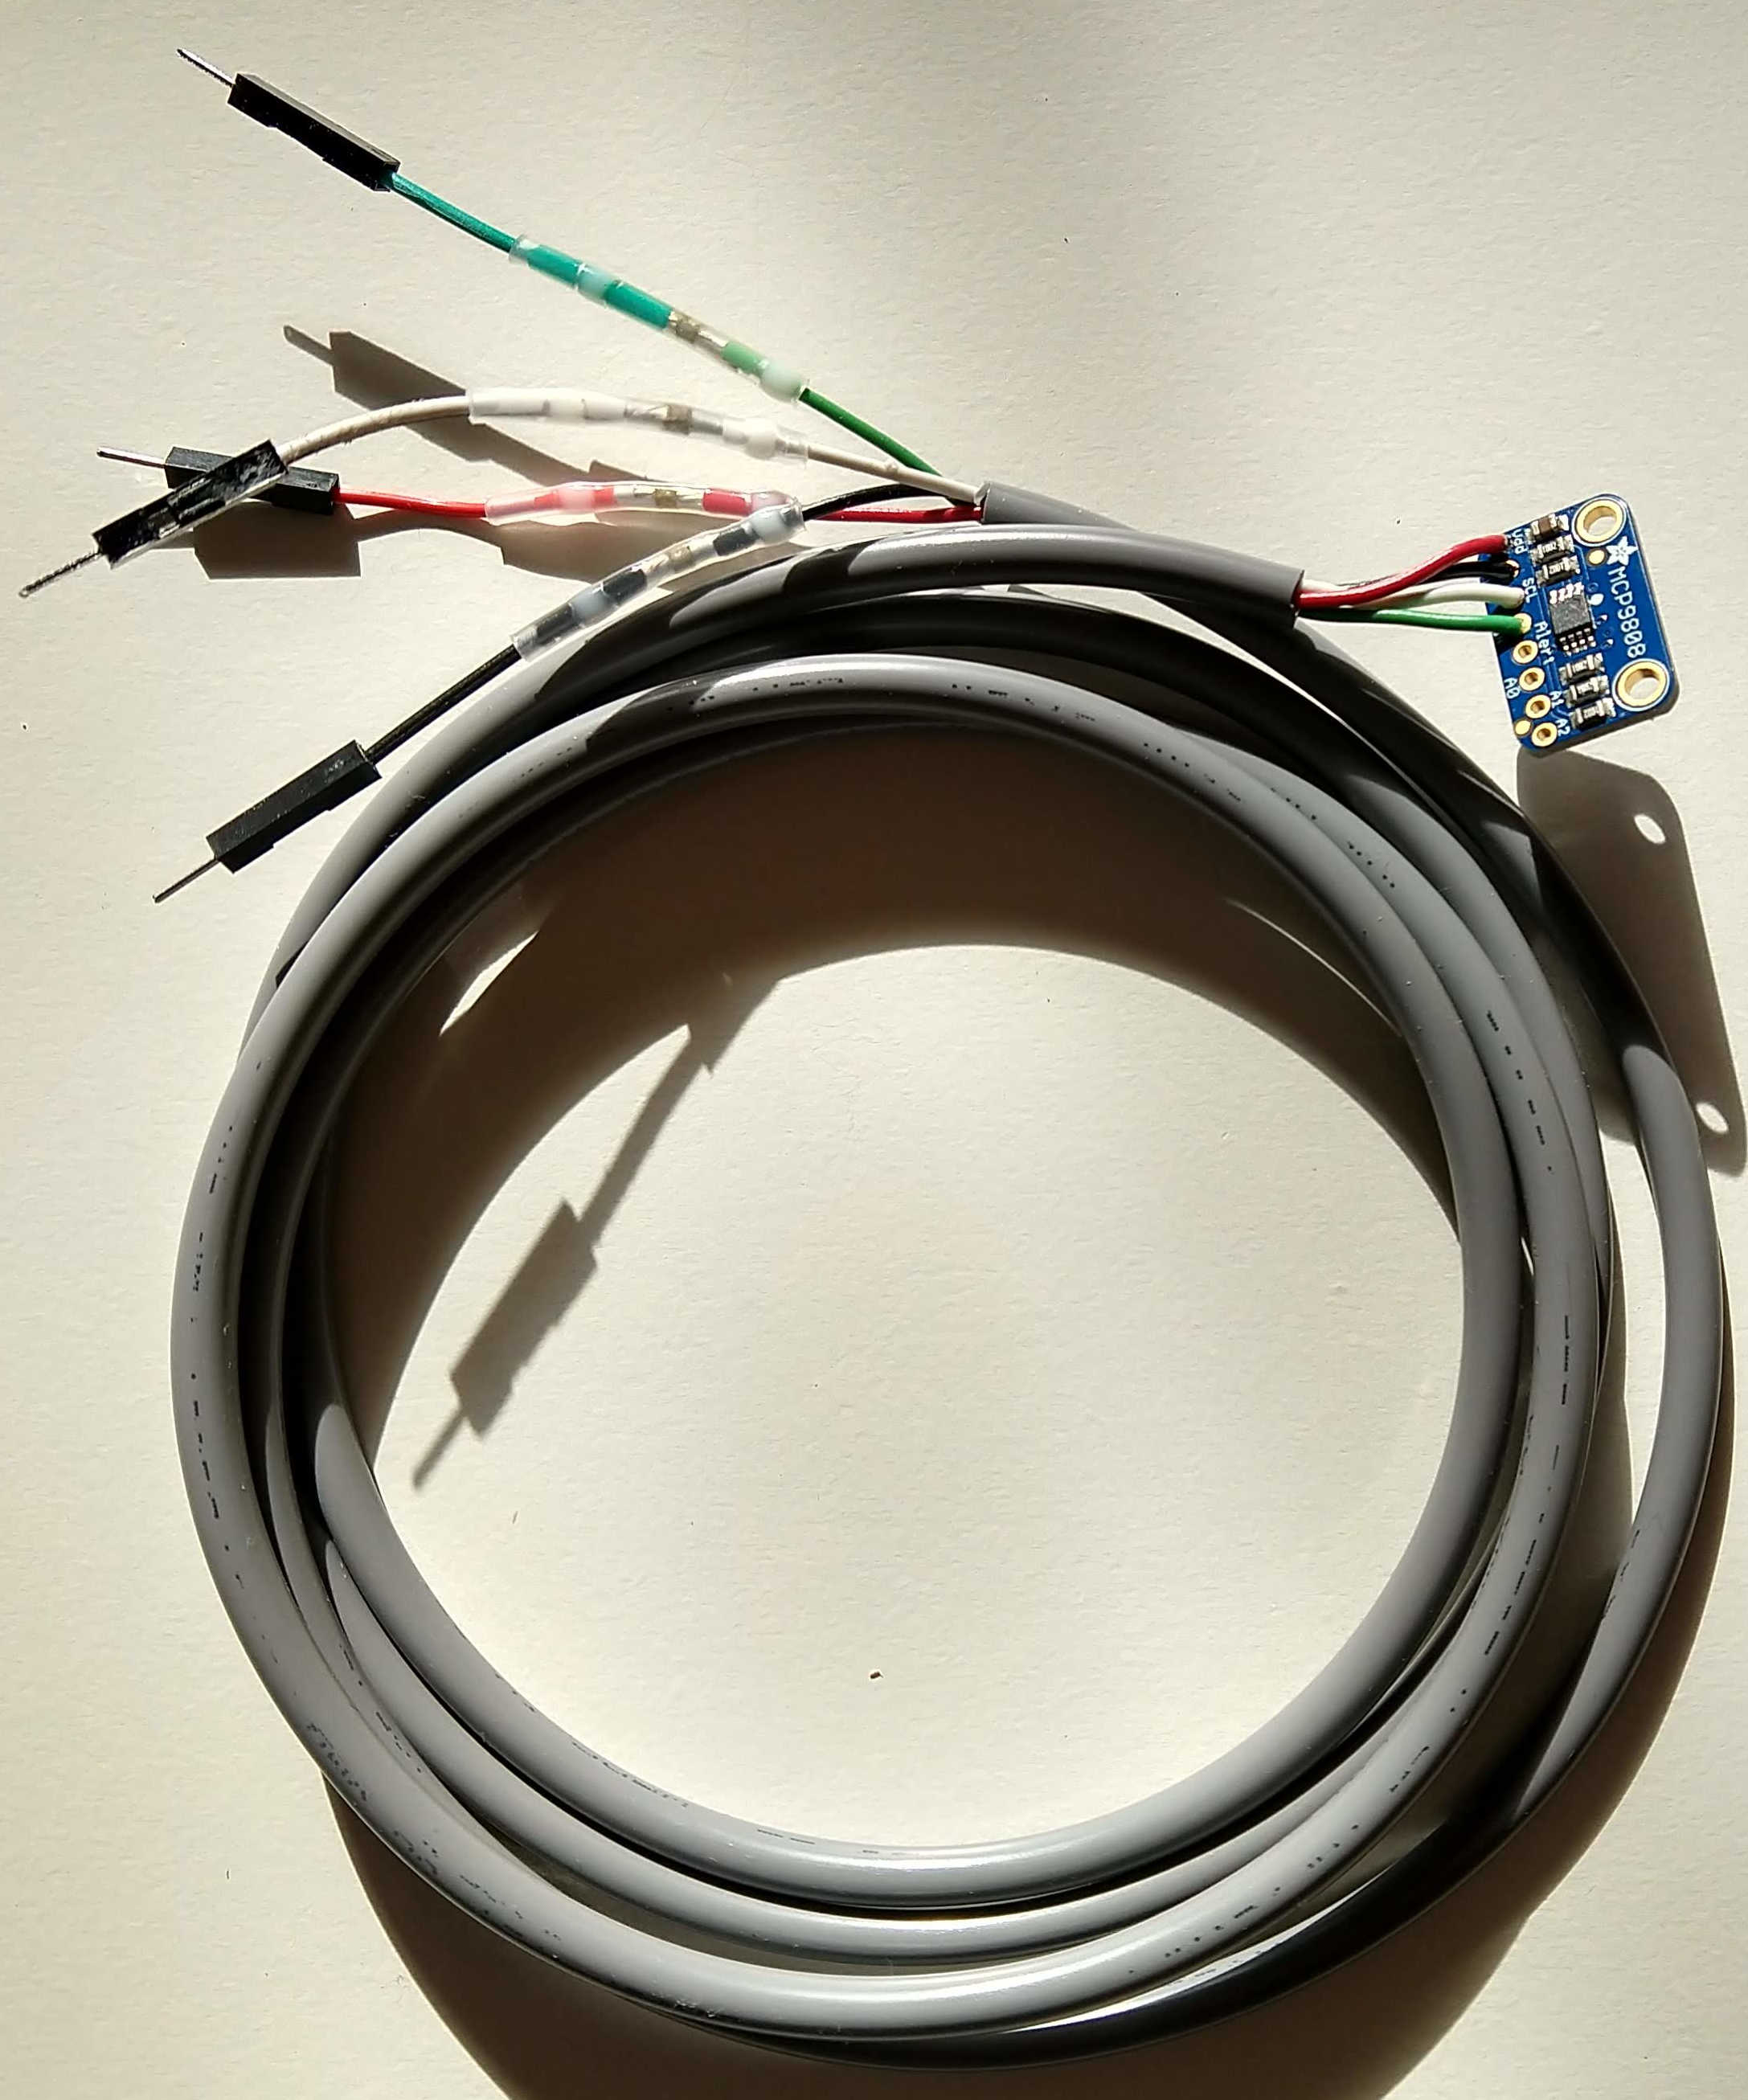
\includegraphics[width=\MFW]{Images/MCP9808_on_cable_cropped.jpg}}{https://github.com/publicsensors/IntroSensors/blob/digital/Images/MCP9808_on_cable_cropped.jpg}
		%\includegraphics[height=5cm]{Images/DS3231breadboard.jpg}
		\caption[MCP9808 on breadboard]{An \MCP9808 temperature sensor soldered onto a cable with 4 conductors (red $\leftrightarrow$ \texttt{Vdd}, black $\leftrightarrow$ \texttt{GND}, white $\leftrightarrow$ \texttt{SCL} and green $\leftrightarrow$ \texttt{SDA}).
		Male jumper ends are connected to the other end of the cable with \glspl{ssw_connector}.
		Note that, for clarity, the jumpers on the other end of the cable have colors consistent with the corresponding wires attached to the sensor.}
		\labfig{mcp9808_cable}
	\end{center}
\end{marginfigure}


\begin{marginfigure}
	\begin{center}
		\htmladdnormallink{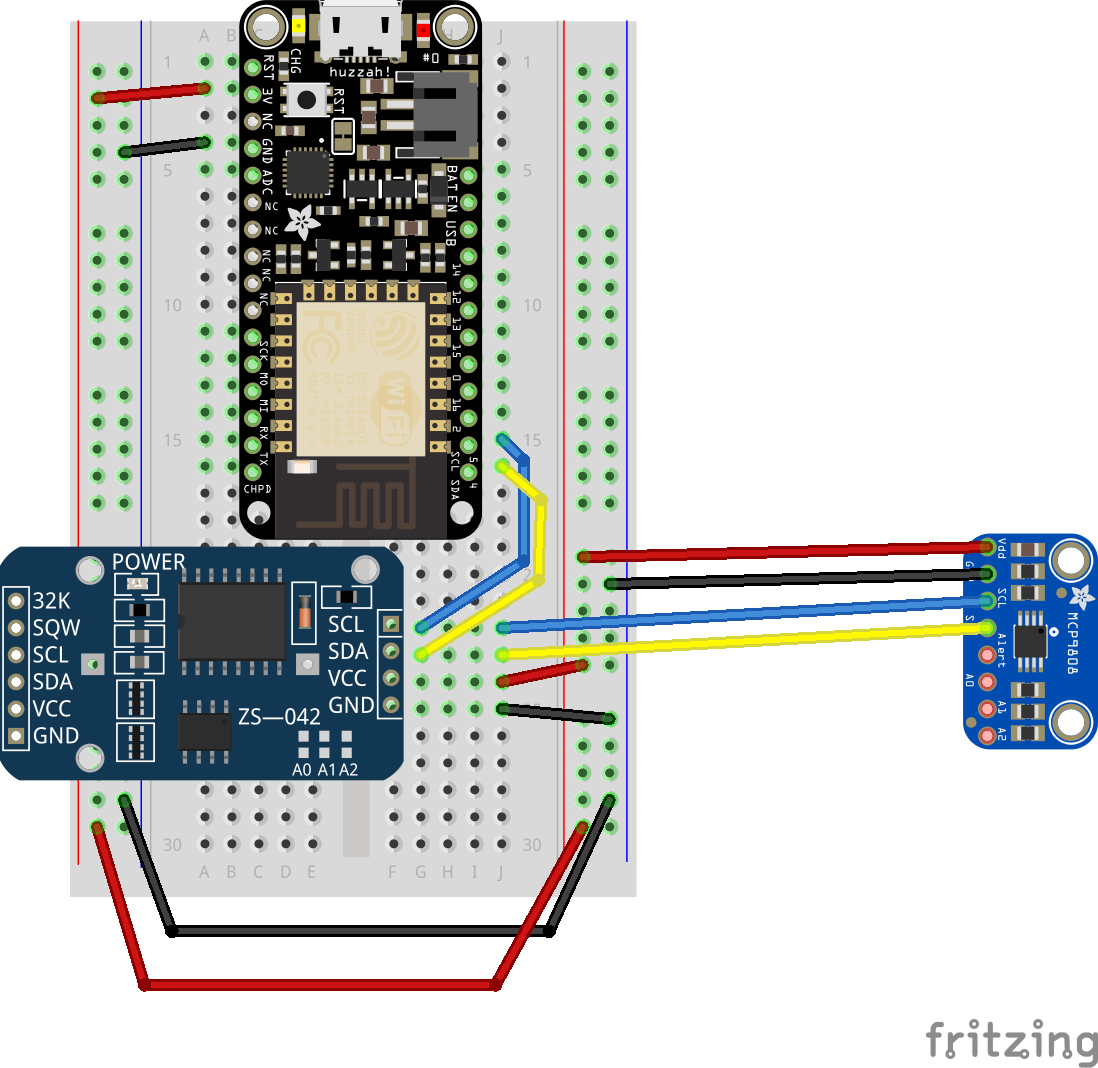
\includegraphics[width=\MFW]{Fritzing/feather_MCP9808_bb.png}}{https://github.com/publicsensors/IntroSensors/blob/digital/Fritzing/feather_MCP9808_bb.png}
		%\includegraphics[height=5cm]{Images/DS3231breadboard.jpg}
		\caption[MCP9808 on breadboard]{An example of layout and wire connections for the \MCP9808 temperature sensor and ESP8266 microcontroller. The circuit layout is similar to that used for the DS3231 external Real Time Clock. The DS3231 is left in the figure to emphasize that \i2c can support multiple devices simultaneously, but this exercise works equally well with or without the DS3231.}
		\labfig{mcp9808_breadboard}
	\end{center}
\end{marginfigure}


\begin{enumerate}
	\item \textbf{Connect wires to the GND, Vdd, SCL and SDA pins on the \MCP9808}.

	Like in the thermistor calibration in \refsec{cal_therm}, we will use ``water baths'' made of paper cups to expose the \MCP9808 sensors to known temperatures without getting them wet.
	This is most easily done if the sensor is connected to the microcontroller by extra long wires.

	\smallskip
	If your \MCP9808 has pins soldered to it, you can use two or more jumpers attached in series to give enough scope to move the sensor around.
	If your sensor does not have pins, you can solder some on, or alternatively solder long wires directly to the sensor (\reffig{mcp9808_cable}).

	You can then connect the other ends of the wires to the breadboard by soldering pins or male jumpers onto them; \reffig{mcp9808_cable} shows an example of this.
	The cable in this figure was made with \glspl{ssw_connector}, a fast and convenient way to join and protect two wire ends.

	Alternatively, you can attach wires directly to terminals (\eg, like \htmladdnormallink{these}{https://www.adafruit.com/product/2137?gclid=CjwKCAjwq9mLBhB2EiwAuYdMtZGP6ggrSAALQm8J7sbJ8Mwr6zWCWucqFVLvuSnaAGO22bPzFGNxmhoCVvEQAvD_BwE}), that then insert into breadboards.


	\item \textbf{Connect the GND and 3V pins on the ESP8266 to the GND and Vdd pins on the \MCP9808}.

	The circuit layout for the \MCP9808 is shown in \reffig{mcp9808_breadboard}.


	\item Connect the \texttt{SDA} (\#4) pin on the ESP8266 to the \texttt{SDA} pin on the \MCP9808, and the  \texttt{SCL} (\#5) pin on the ESP8266 to \texttt{SCL} on the \MCP9808.
	\item \textbf{Download the driver module provided on github by \texttt{@kfricke} called \htmladdnormallink{mcp9808.py}{https://raw.githubusercontent.com/kfricke/micropython-mcp9808/master/mcp9808.py} for the \MCP9808 temperature sensor.}

	Save it into a \texttt{Codes} directory on your computer.

	\item \textbf{Copy } \lstinline{mcp9808.py} \textbf{onto your microcontroller, using \thonny, \texttt{WebREPL} or \mpfshell (see the methods from \refch{connect} if you have questions).}
	\item %You are now ready to test your \DS3231 \rtc.
	\textbf{Set up the \i2c connection to your \MCP9808:}
\begin{lstlisting}[language=Python]
from machine import I2C, Pin
import mcp9808

i2c=I2C(scl=Pin(5),sda=Pin(4))
temp_mcp9808=mcp9808.MCP9808(i2c=i2c)
\end{lstlisting}
	\item \textbf{Set the resolution on your \MCP9808 to the highest possible}, with:
\begin{lstlisting}[language=Python]
temp_mcp9808.set_resolution(mcp9808.TEMP_RESOLUTION_MAX)
\end{lstlisting}

	\item \textbf{Query the temperature from your \MCP9808}:

	Here, there are two choices:
	If your microcontroller can do floating point math, use
\begin{lstlisting}[language=Python]
temp_mcp9808.get_temp()
\end{lstlisting}
The result of this command is the temperature in degrees Celsius, expressed as a floating point number.

\smallskip
If your microcontroller cannot do floating point math, use
\begin{lstlisting}[language=Python]
temp_mcp9808.get_temp_int()
\end{lstlisting}
The result of this command is two numbers.
The first is the temperature in whole degrees Celsius, expressed as an integer.
The second is the remaining fraction of a degrees Celsius, expressed as another integer.

\end{enumerate}
\loadMilestone{mlst:05a} % load milestone with tags id: mlst:04c


\subsection{\color{gray} Multiple sensors on a device: Temperature and pressure on an MS5803 \color{black}}

\subsection{Resolving \i2c address conflicts with a multiplexer}
\labsec{i2c_multi}
The requirement that each device on an \i2c bus has a unique address sometimes leads to address conflicts, in which two or more sensors have the same address.
Sometimes it is possible to create additional \i2c buses, dividing the duplicated address between them.
However, this is often not practical, especially when more than two devices share an address or when the number of \texttt{GPOI}s is limited.
Some \i2c devices have two or more addresses, which can be selected using jumpers between pins on the devices.
Altering one sensor's address in this way is often a workable solution to address conflicts.
However, many \i2c sensors have fixed addresses.
Furthermore, in an instrument designed to operate in the environment, sensors are often ``potted'' in epoxy or a sealant, or otherwise enclosed to protect them from water, salt, dust, \etc
These sensors typically are difficult or impossible to access to alter pin connections that shift \i2c addresses.

In these cases, an alternative strategy is provided by an \i2c \emph{multiplexer}.
An \i2c multiplexer is an \i2c device, which creates several (typically 8) \i2c ``sub-buses''.
The multiplexer allows i2c communications from only one sub-bus at a time -- which one is determined by a software command sent to the multiplexer by the microcontroller.
This means that two \i2c devices can be on different sub-buses, and because only one is operating at a given time there is no conflict even if they share the same address.

The details are best conveyed by an example:

The effect of light energy on many biological and physical processes is strongly affected by from which part of the spectrum it comes -- that is, it's \texttt{color}, taken to include wavelengths invisible to humans such as \gls{irLabel} and \gls{uvLabel}.
Under water, in forest canopies, at dawn or dusk or at high latitudes, and in many other situations it is potentially important to characterize light intensity as a function of color.
A \htmladdnormallink{TCS34725}{https://cdn-shop.adafruit.com/datasheets/TCS34725.pdf} color sensor, such as \htmladdnormallink{this one made by Adafruit}{https://www.adafruit.com/product/1334}, measures the \htmladdnormallink{RGB}{https://en.wikipedia.org/wiki/RGB_color_model} components of incident light.
However, to accurately characterize these primary colors, its light sensors are equipped with optical filters that exclude \gls{irLabel} wavelengths.
The \htmladdnormallink{TSL2591}{https://cdn-learn.adafruit.com/assets/assets/000/078/658/original/TSL2591_DS000338_6-00.pdf?1564168468} color sensor, such as \htmladdnormallink{also made by Adafruit}{https://www.adafruit.com/product/1980}, measures both full spectrum light intensity and the \gls{irLabel} component of that intensity.
So, simultaneous readings from both these sensors would characterize the blue, green, red and \gls{irLabel} component light intensities.

However, these sensors share the same \i2c address, so both cannot function simultaneously on the same \i2c bus.

\subsubsection{\howto Set up a TCA9548A \i2c multiplexer}

\begin{marginfigure}[-14cm]
	\begin{center}
		\htmladdnormallink{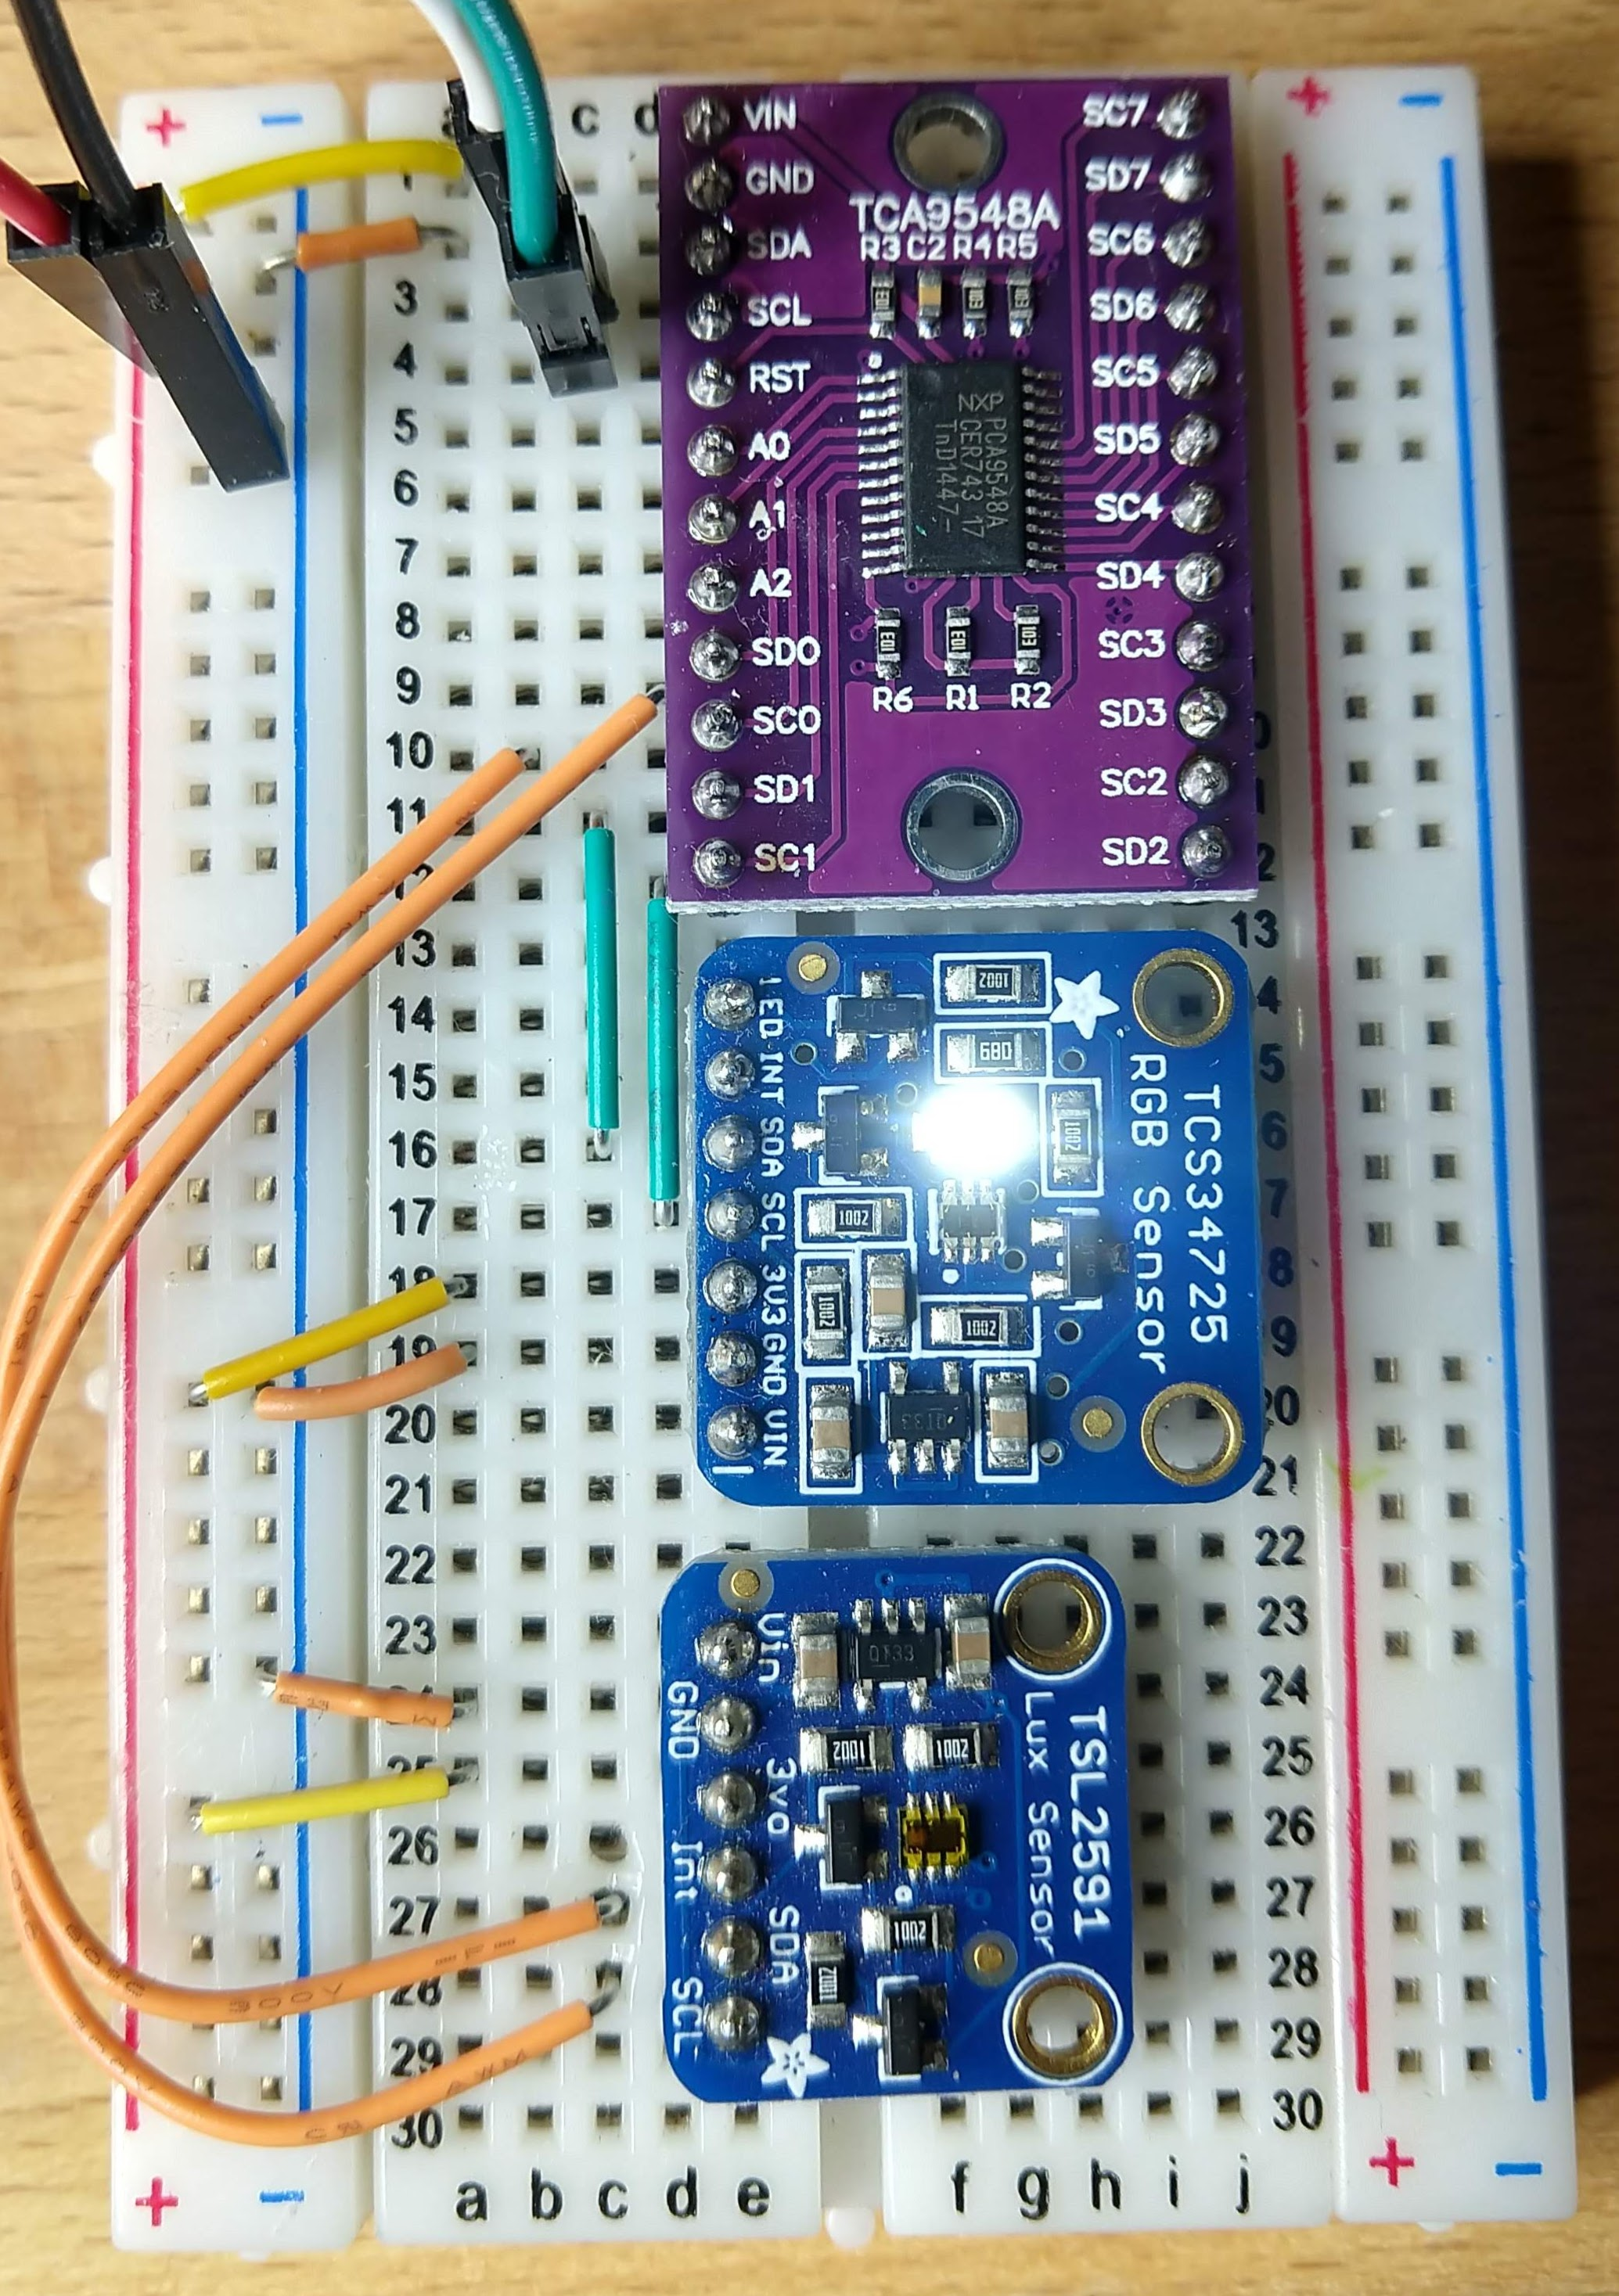
\includegraphics[width=\MFW]{Images/i2c_multiplexer_circuit.jpg}}{https://github.com/publicsensors/IntroSensors/blob/digital/Images/i2c_multiplexer_circuit.jpg}
		\caption[TCA9548A \i2c multiplexer circuit]{A TCA9548A \i2c multiplexer is used in this circuit to enable both a TCS34725 color sensor and a TSL2591 full spectrum/\gls{irLabel} sensor to operate on the same \i2c bus, even though they share the same \i2c address. The jumpers at the upper left lead to the microcontroller (red $\leftrightarrow$ \texttt{3V3}, black $\leftrightarrow$ \texttt{GND}, white $\leftrightarrow$ \texttt{SCL} and green $\leftrightarrow$ \texttt{SDA}. The white dot at the center is the built-in LED on the TCS34725, used to provide a standard illumination spectrum in some types of color measurements.}
		\labfig{i2c_mulitplx}
	\end{center}
\end{marginfigure}

A solution using a TCA9548A \i2c multiplexer is shown in \reffig{i2c_mulitplx}.
To use this circuit, we can use a modification of code posted on the \htmladdnormallink{MicroPython forum}{https://forum.micropython.org/viewtopic.php?t=6284} as a driver for the TCA9548A:
\lstinputlisting[language=Python,label=TCA9548Adriver,caption={\htmladdnormallink{\texttt{tca9548a.py}}{https://github.com/publicsensors/IntroSensors/blob/main/Codes/tca9548a.py}: A short driver for the TSC9548A \i2c multiplexer.}]{Codes/tca9548a.py}
% \lstinputlisting[language=Python,label=SetTimeDS3231,caption={\htmladdnormallink{\texttt{SetTimeDS3231.py}}{https://github.com/publicsensors/IntroSensors/blob/main/Codes/SetTimeDS3231.py}: A Micropython utility to set a \DS3231 \rtc to time from a Network Time Protocol (NTP) server.}]{Codes/SetTimeDS3231.py}

The TCS34725 color and TSL2591 full spectrum/\gls{irLabel} sensors as laid out in the circuit in \reffig{i2c_mulitplx} can then be querried with the following code:
\lstinputlisting[language=Python,label=I2Cmultiplexer,caption={\htmladdnormallink{\texttt{multiplex\textunderscore i2c.py}}{https://github.com/publicsensors/IntroSensors/blob/main/Codes/multiplex_i2c.py}: An example use of  a TCA9548A \i2c multiplexer to communicate with color and full spectrum/\gls{irLabel} sensors that have an \i2c address conflict.}]{Codes/multiplex_i2c.py}

Note that this code imports the drivers for the TSC34725 color sensor, \htmladdnormallink{tsc34725.py}{https://github.com/adafruit/micropython-adafruit-tcs34725}, and for the TSL2591 full spectrum/\gls{irLabel} sensor, \htmladdnormallink{tsl2591.py}{https://github.com/jfischer/micropython-tsl2591}, assuming both have been copied onto the microcontroller.

The output of this demonstration code is:
\begin{lstlisting}[language=Python]
>>> import multiplex_i2c
light_sample =  628.646
color_sample =  (15, 10, 9, 34)
light_sample =  628.646
color_sample =  (15, 10, 9, 34)
light_sample =  628.646
color_sample =  (15, 10, 9, 34)
light_sample =  628.646
color_sample =  (15, 10, 9, 34)
light_sample =  628.646
color_sample =  (15, 10, 9, 34)
light_sample =  628.646
color_sample =  (15, 10, 9, 34)
light_sample =  64.464
color_sample =  (3, 1, 1, 5)
light_sample =  121.91
color_sample =  (4, 2, 2, 7)
light_sample =  121.91
color_sample =  (4, 2, 2, 7)
light_sample =  628.646
color_sample =  (15, 10, 9, 34)
>>>
\end{lstlisting}

\loadMilestone{mlst:05b} % load milestone with tags id: mlst:04c

\subsection{Using I2C over long cables with differential extenders}
\labsec{i2c_extend}

\begin{marginfigure}
	\begin{center}
		\htmladdnormallink{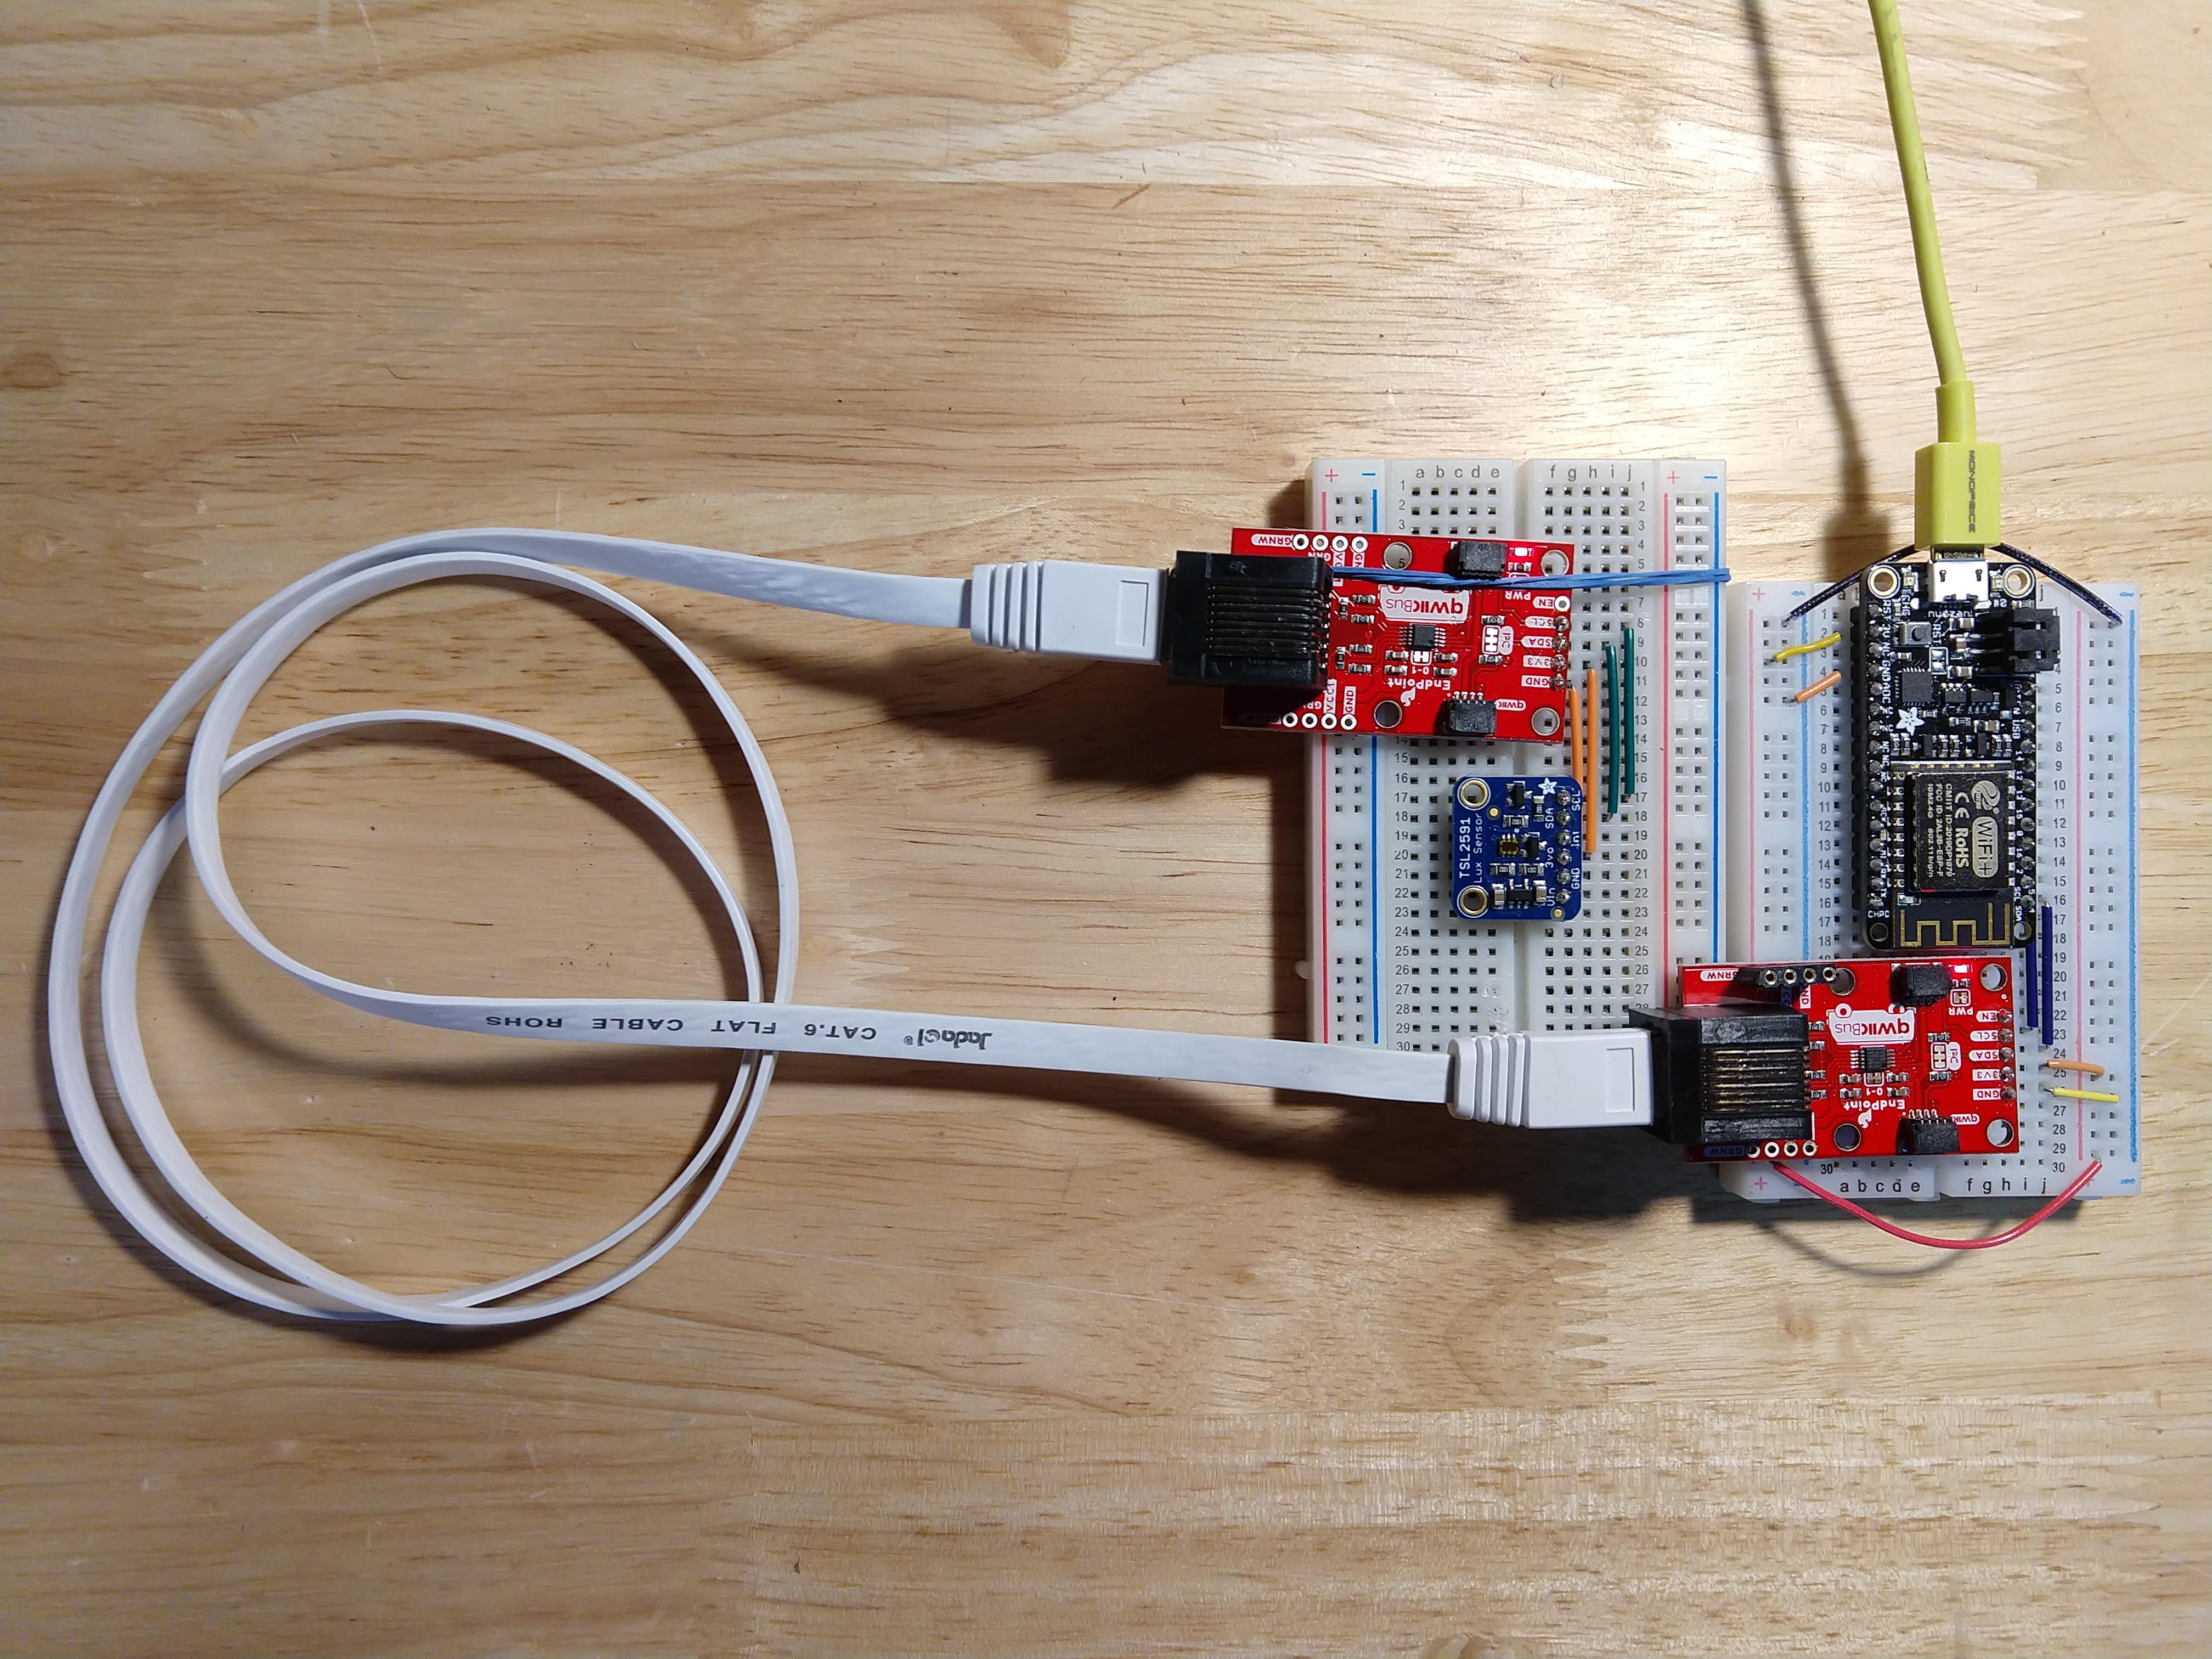
\includegraphics[width=\MFW]{Images/I2C_extender2.jpg}}{https://github.com/publicsensors/IntroSensors/blob/digital/Images/I2C_extender2.jpg.jpg}
		%\includegraphics[height=5cm]{Images/DS3231breadboard.jpg}
		\caption[PCA9615-based differential \i2c extender layout]{A PCA9615-based differential \i2c extender using two \htmladdnormallink{QwiicBus Endpoints}{https://www.sparkfun.com/products/16988}, connecting a microcontroller and a \texttt{TSL2591} light sensor via a CAT-5 ethernet cable.}
		\labfig{i2c_ext}
	\end{center}
\end{marginfigure}


\i2c was originally designed to operate over short distances, e.g., between a sensor and a microprocessor on the same circuit board.
However, its use has broadened considerably, and in the context of environmental sensors it can be very useful to place sensors at a distance from the microcontoller that reads them.
Examples include sensors that are underwater, in soil, or in electrically noisy environments where a microcontroller would either not survive or not be accessible to program or download data.

The effective cable length over which \i2c can reliably operate depends on the details of the devices and conductors used, the type and intensity of electrical noise in the vicinity, and parameter settings such as clock rate.
In many situations in which noise or cable length makes ordinary \i2c connections unreliable, using \texttt{differential extenders} to span all or most of the relevant distances may be a practical solution.
Differential extenders use pairs of wires for both \texttt{SDA} and \texttt{SCA}, with the signal encoded as the voltage difference between the two wires in each pair.
A typical conductor is an ethernet cable, which has four twisted conductor pairs.
The rationale is that noise which affect one wire in a pair will affect the other almost identically.
The voltage difference between paired wires is therefore much less sensitive to noise than an isolated wire, as is used in ordinary \i2c layouts.

An example is Sparkfun's \htmladdnormallink{QwiicBus}{https://learn.sparkfun.com/tutorials/sparkfun-qwiicbus-hookup-guide} system, which is based on a \texttt{PCA9615} integrated circuit (see the \htmladdnormallink{datasheet}{https://cdn.sparkfun.com/assets/a/5/1/3/6/PCA9615.pdf}).
\reffig{i2c_ext} is an example of a circuit layout using two \htmladdnormallink{QwiicBus Endpoints}{https://www.sparkfun.com/products/16988} to connect an \esp8266 microcontoller on one breadboard to an \i2c light sensor on a different breadboard.

In this example the connecting cable is only 3 feet long.
However, Sparkfun claims these devices can operate across cables over 100 feet long, and (as described later in this textbook) direct burial ethernet cable lends itself well to weather- and water-proofed environmental sensor installations.

\begin{kaobox}[frametitle=Potential for change \dots]
There is another situation in which using a differential extender: when different parts of an \i2c circuit must operate at different voltages.
An example is an \texttt{ADS1115} voltage sensor.
The maximum voltage tolerance of this sensor is determined in part by the voltage at which it is powered.
An \texttt{ADS1115} operating at 5V has a higher maximum voltage than the same sensor operating at 3.3V.
However, the \gpios on most modern microcontrollers (including the \esp8266) operate only at 3.3V.

Using a differential extender based on \texttt{PCA9615}'s makes it possible to have the part of the \i2c bus directly connected to the microcontroller operate at 3.3V, while the part indirectly connected through the extender (e.g., the \texttt{ADS1115}) operates at 5V or higher voltage.
Some other types of extenders may also have similar capabilities.
This is accomplished by cutting traces on the upstream extender, and adding jumpered connections for ground and input voltage, as described in detail on \htmladdnormallink{Sparkfun's documentation}{https://learn.sparkfun.com/tutorials/sparkfun-qwiicbus-hookup-guide}.
\end{kaobox}


\loadMilestone{mlst:05d} % load milestone with tags id: mlst:04c

\subsection{Using System Management Bus (\smbus) devices}
\labsec{i2c_smbus}
The \htmladdnormallink{System Management Bus}{https://en.wikipedia.org/wiki/System_Management_Bus}, or \smbus, is a digital interface protocal derived from \i2c that is used in some devices useful for environmental sensing.
For most purposes relevant to environmental sensing, \smbus differs from \i2c primarily in the \Micropython library used to communicate with sensors.
Unlike \i2c, \smbus is not installed by default in \Micropython firmware.
However, \verb|@gkluoe| has provided code that simulates an \smbus interface at his \htmladdnormallink{github site}{https://github.com/gkluoe/micropython-smbus}.

Because these protocols are similar, it is usually possible to combine \i2c and \smbus devices on the same bus, addressing each sensor using the appropriate library.

An example is provided by a \htmladdnormallink{Hardkernel Weatherboard 0.2}{https://www.hardkernel.com/shop/weather-board-2/}.
This board combines two sensors: a \texttt{BME280} sensor, using an \i2c interface to measure humidity, temperature and barometric pressure (including altitude); and, a \texttt{SI1132} sensor, using an \smbus interface to measure ambient and ultraviolet (UV) light.

\subsubsection{\howto Combine \i2c and \smbus sensors on a single bus}
\begin{enumerate}
	\item \textbf{Connect wires from the GND, 3.3V, SCL and SDA pins on your microcontroller to the Weatherboard}.

	Note that, on the Weatherboard, the 3.3V pin is labelled \texttt{P3V45}.

	\item \textbf{Copy drivers onto your microcontroller}.

	The necessary drivers are:
	\begin{itemize}
		\item \htmladdnormallink{bme280\_float.py}{https://raw.githubusercontent.com/publicsensors/IntroSensors/digital/Codes/bme280_float.py}, for the \texttt{BME280} sensor;
		\item \htmladdnormallink{si1132.py}{https://raw.githubusercontent.com/publicsensors/IntroSensors/digital/Codes/si1132.py}, for the \texttt{SI1132} sensor;
		\item The \htmladdnormallink{usmbus folder}{https://github.com/publicsensors/IntroSensors/tree/digital/Codes/usmbus}, providing the \smbus library.
	\end{itemize}
	Here, we are using a version of the Python driver for the \texttt{SI1132} sensor provided by \htmladdnormallink{ControlEverythingCommunity}{https://github.com/ControlEverythingCommunity/SI1132} that has been modified to use the \texttt{usmbus} \smbus emulator.

	\item \textbf{Import the drivers, initialize the sensor objects and create a loop for sampling}.

	The \texttt{BME280} and \texttt{SI1132} can then be querried with the following code:
\lstinputlisting[language=Python,label=test_bme280_si1132,caption={\htmladdnormallink{\texttt{test\textunderscore bme280 \textunderscore si1132.py}}{https://github.com/publicsensors/IntroSensors/blob/main/Codes/test_bme280_si1132.py}: Test code demonstrating simultaneous use of \i2c and \smbus devices: \texttt{BME280} and \texttt{SI1132} sensors on a \htmladdnormallink{Hardkernel Weatherboard 0.2}{https://www.hardkernel.com/shop/weather-board-2/}.}]{Codes/test_bme280_si1132.py}

The output of this code should be something like:
\begin{lstlisting}[language=Python]
>>> import test_bme280_si1132

bme280:  ('19.59C', '990.11hPa', '49.29%')
si1132 uv, ir, visible = 3, 260, 262 lux

bme280:  ('19.54C', '990.05hPa', '48.58%')
si1132 uv, ir, visible = 2, 261, 260 lux

bme280:  ('19.54C', '990.09hPa', '48.63%')
si1132 uv, ir, visible = 2, 259, 261 lux

bme280:  ('19.53C', '990.06hPa', '48.57%')
si1132 uv, ir, visible = 2, 260, 260 lux
\end{lstlisting}

\end{enumerate}

\newpage

\section{1-wire sensors}
\labsec{1wire_sensors}
\subsection{Background}
1-wire is a proprietary protocol design that, as the name implies, uses only one wire in addition to \texttt{Vin} and \texttt{GND}.
1-wire is used in relatively few sensor types, but is worth knowing about because one of those is an inexpensive and versatile \htmladdnormallink{temperature sensor}{https://datasheets.maximintegrated.com/en/ds/DS18B20.pdf} that is among the most useful available for environmental monitoring.

\smallskip
1-wire supports many (up to hundreds) of devices on a single cable, each of which can be independently queried for sensor readings because it has a unique 64-bit ROM address.
1-wire supports lower (but still generally sufficient) data rates than \i2c, which (when properly configured) can operate over much longer cables.

\subsection{Temperature measurements with \texttt{DS18B20} digital sensors}
The \texttt{DS18B20} device consists of an internal temperature sensor based on a temperature dependent resistor, a small processor for converting the signal into digital form, some power management circuitry, and memory used to store the device's unique 64-bit ROM identifier.
After the built-in sensor on makes a temperature measurement, it communicates the result digitally, using the 1-wire protocol.
The \texttt{DS18B20}'s use of the 1-wire protocol makes it extremely simple to connect one or more of these devices to a microcontroller.
All that is required is to provide 3.3V power, ground, and the data connection, each of which can be shared by many \texttt{DS18B20} sensors.  

\begin{marginfigure}[0cm]
	\begin{center}
		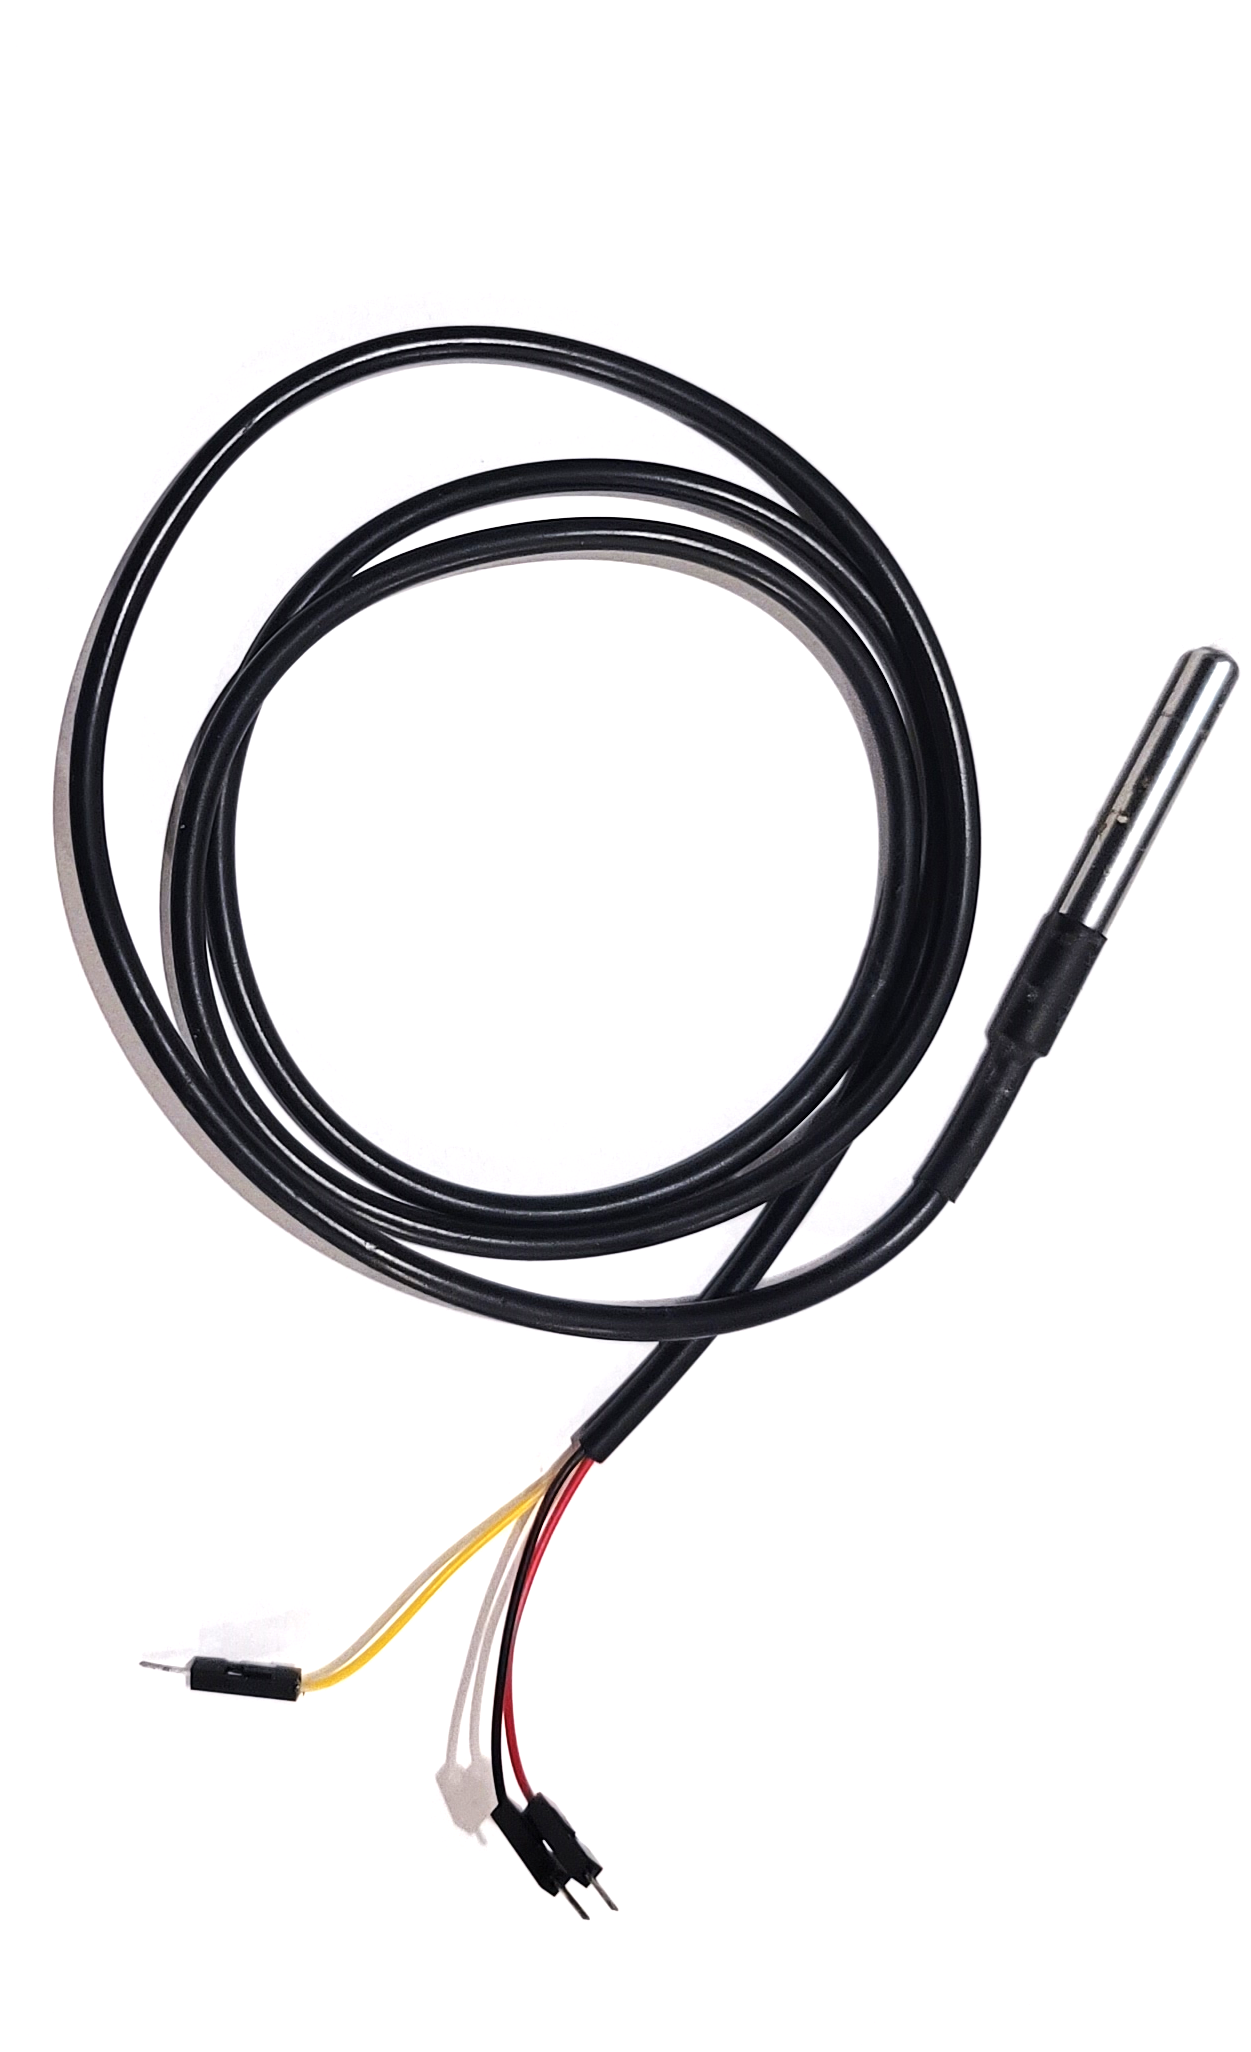
\includegraphics[height=7cm]{Images/waterproofDS18B20.png}
		\caption[Waterproofed DS18B20]{A waterproof version of the \texttt{DS18B20} temperature sensor.}
		\labfig{waterproofDS18B20}
	\end{center}
\end{marginfigure}


The \texttt{DS18B20} sensor has a temperature range of -55\textdegree C and +125\textdegree C, and can be powered at VDD between 3V and 5.5V. Error tends to be between 0.5 \textdegree C and 2 \textdegree C, depending on the temperature, but this can be improved to some extent with calibration.
The sensor is available at very low cost (often under \$1 U.S.) in a number of form factors, some of which include weatherproofing and a pre-installed cable \reffig{waterproofDS18B20}.
Most official releases of \Micropython include a build-in library that provides access to the driver for the \texttt{DS18B20} temperature sensor.
The low cost, reasonably good accuracy, and ease of use make them ideal for environmental temperature characterization.

Detailed commands necessary for communicating with this sensor are described in the \htmladdnormallink{\texttt{DS18B20}}{Onewirehttps://docs.micropython.org/en/latest/esp32/quickref.html?highlight=dht\#onewire-driver} section of the \Micropython docs.  The example provided here follows the tutorial closely.

The onewire and ds18x20 libraries provide access to functions required to use the device.  These must be imported before communicating with the sensor. We'll also need to impore the \texttt{machine} library so that we can access to the microcontroller's pin-related functions and the time libary so that we can insert pauses into the loop we use to interface with the sensor.

\begin{lstlisting}[language=Python]
import onewire, ds18x20
import machine
import time
\end{lstlisting}

\begin{marginfigure}[-1cm]
	\begin{center}
		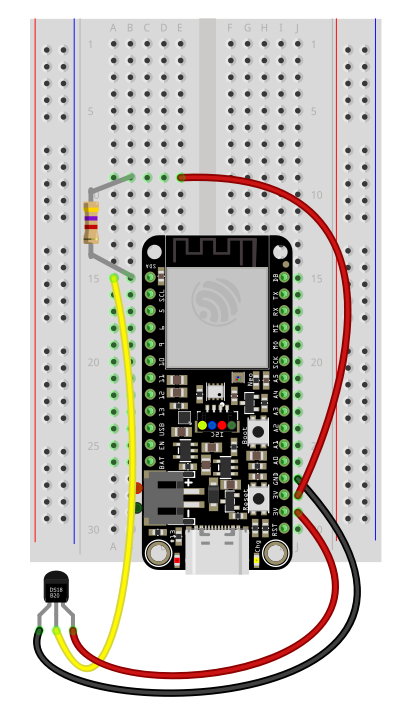
\includegraphics[height=9cm]{Images/singleDS18B20.png}
		\caption[Single DS18B20 on breadboard]{Connecting a single \texttt{DS18B20} temperature sensor to a Feather-based microcontroller.
If the yellow data line is connected to a microcontroller pin that includes a built-in pull-up resistors, the external resistor is not required.}
		\labfig{singleDS18B20}
	\end{center}
\end{marginfigure}
  
To try your sensor, hook up the power wire (red on most waterproofed versions of the \texttt{DS18B20} to the 3.3V pin the microcontroller, the ground wire (black on waterproofed versions) to the ground pin, and the signal wire (yellow on waterproofed versions) to any GPIO pin, as illustrated in \reffig{singleDS18B20}. 


The MicroPython documentation recommends connecting a 4,700 Ohm resistor between the data and power pins, but anything between 2,000 to about 10,000 ohm will probably work. 
The purpose of the resisor is to ensure that the default voltage state of the communication line is positive.  
Pull-up resistors like this are often required on digital communication lines, particularly lines that use the I2C protocol.  
Because they are so frequently required, many microcontroller breakout boards include pull-up reisistors on certain pins.  
On the \texttt{Adafruit} Feather ESP32-S2 board, both the SDA and SCL pins (which correspond to \texttt{GPIO} Pins 3 and 4, respectively) include built-in pull-up resistors. 
Other microcontroller boards may include pull-up resistors on other pins--a quick review of the datasheet board's documentation usually allows such pins to be identified.  
\sidenote[][2cm]{
	\begin{kaobox}[backgroundcolor=\SNcolor,frametitlebackgroundcolor=\SNcolor,frametitle=Idenfity pins with built-in pull-up resistors]
	Many, but not all, microcontroller boards include pull-up resistors on the SCL and SDA pins.  To check if this is the case, either consult the documentation for the board (schematics are particularly helpful) or simply disconnect the microcontroller from all power and external devices and use a multimeter to measure the resistance between a given pin and the 3.3V pin on the board. A resistance measurement in the 1000s of Ohms indicates that the pin likely includes a pull up resistor. In addition,  pins connected to built-in LEDs that are enabled when the pin is set to a low-level logic state normally have pull-up resistors attached.  
	\end{kaobox}
}
 
Now , create an object that can be used to access the data line.

\begin{lstlisting}[language=Python]
dat = machine.Pin(3, machine.Pin.PULL_UP)
\end{lstlisting}

Here, we are using SCL pin on the \texttt{Adafruit} ESP32 Feather-S2 board. 
Calling with the Pin.PULL\textunderscore UP argument is not strictly necessary because the pin already includes the pull-up resistor, but using this argument can sometimes allow a high-value resistor internal to the ESP chips to provide sufficent pull that the sensor will work in the absence of a physical pull-up resistor.

Now create an instance of the onewire object on the dat pin and use functions defined in the library for this object to see whether any devices are connected and to return a unique identifier (in "byte-array" format—which will be displayed as hexadecimal numbers, same as last week) for each sensor in the variable roms (a Python list), and then print these identifiers to the screen:  

\begin{lstlisting}[language=Python]
ds = ds18x20.DS18X20(onewire.OneWire(dat))
\end{lstlisting}

Now scan for all 1-wire devices that are connected to the data line and record the 64-bit ROM identifier to a list named (obviously enough) roms.

\begin{lstlisting}[language=Python]
roms = ds.scan()
print("found devices:", roms)
\end{lstlisting}

All  \texttt{DS18B20} sensors on the data line listen for the command that tells them to do a temperature reading (the .convert\textunderscore temp() function).
Once the reading is taken, they are ready to send the reading back to the microcontroller whenever the microcontroller calls the .read\textunderscore temp() function with the appropriate identifier. 
So, if a single sensor is connected to the line, the following code prints out a temperature reading.

\begin{lstlisting}[language=Python]
#for single connected probe only
rom = ds.scan()
ds.convert_temp()
time.sleep_ms(750)
temperature = ds.read_temp(rom[0])
print("temperature: ", temperature)
\end{lstlisting}

\begin{marginfigure}[-2cm]
	\begin{center}
		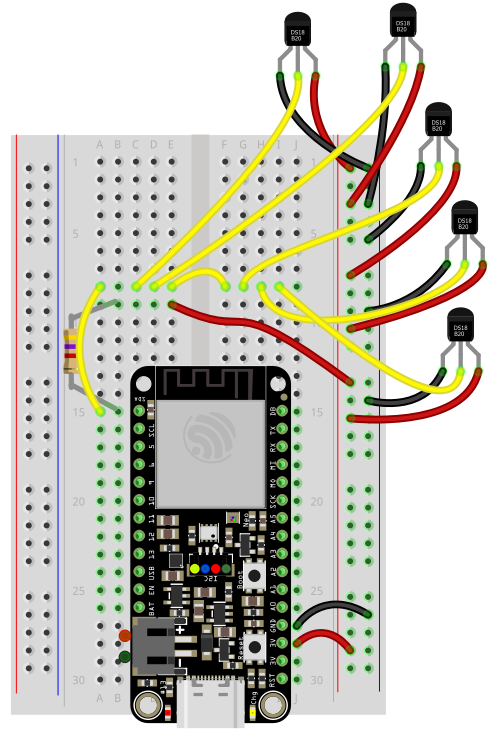
\includegraphics[height=9cm]{Images/fiveDS18B20.png}
		\caption[Five DS18B20 on breadboard]{Connecting five \texttt{DS18B20} temperature sensors in parallel. In this configuration, the data line for all five sensors radiates outward from a single bus.}
		\labfig{fiveDS18B20}
	\end{center}
\end{marginfigure}

\begin{marginfigure}[9 cm]
	\begin{center}
		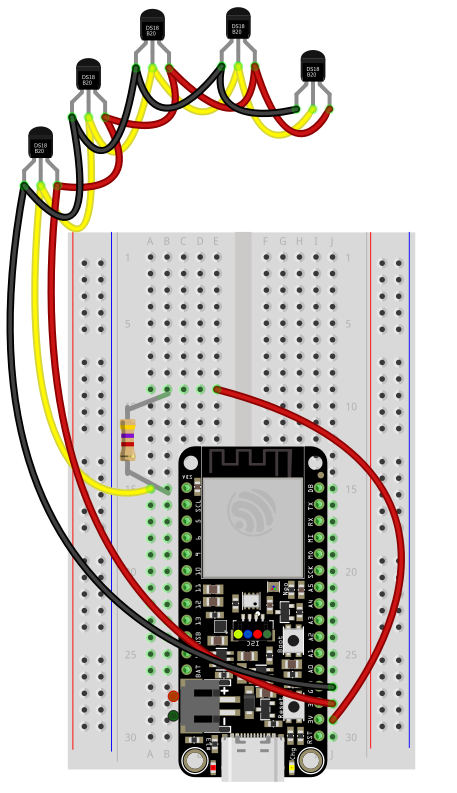
\includegraphics[height=9cm]{Images/fiveDS18B20series.png}
		\caption[DS18B20 daisy chain]{Connecting five \texttt{DS18B20} temperature sensor in daisy-chain fashion.  Here, the connections between sensors are made external to the breadboard.}
		\labfig{fiveDS18B20series}
	\end{center}
\end{marginfigure}

The beauty of the 1-wire protocol is that multiple sensors can be added to the system without making any significant modifications either to hardware or software.
Two different approaches for connecting multiple sensors ares illustrated in \reffig{fiveDS18B20} and \reffig{fiveDS18B20series}. 
In the first, all the sensors are connected directly to a single row of a breadboard.  
The rest of the circuit is identical to that in \reffig{singleDS18B20}. 
In the second approach, the sensors are connected externally to the breadboard daisy-chain fashion.  
The second approach could be used to develop a temperature sensor array that simulaneously collects data from multiple locations.
While both versions can work, note that the DS18B20 documentation advises against sensor network design in which all sensors are a similar distance from a single common bus, so the daisy-chaining approach may be more reliable in adverse conditions such as when there is a large amount of electromagnetic interferane.
In any case, the code for accessing all five sensors is nearly identical to the previous code except that we read the data for each sensor in turn. 

\begin{lstlisting}[language=Python]
#for any number of probes
roms = ds.scan()
ds.convert_temp()
time.sleep_ms(750)
print("temperatures:")  
for rom in roms:
	temperature = ds.read_temp(rom)
	print(temperature)
print()
\end{lstlisting}

Don’t worry too much about the detailed syntax used here—while learning, you’ll usually just cut and paste code to build programs anyway—but do try to get a sense of what each line does.
Basically, the code figures out how many temperature sensors are connected to the pin, triggers the internal temperature measurement in all the sensors,  waits 0.75 seconds (a requirement for the \texttt{DS18B20}), then sequentially communicates with and prints the result from each sensor.

\loadMilestone{mlst:05e} % load milestone with tags id: mlst:05e 

\subsection{\color{gray} Accuracy and precision of DS18B20 temperature sensors \color{black}}
\subsubsection{\color{gray} Improve the accuracy and precision of DS18B20 temperature measurements with recalibration \color{black}}
\subsubsection{\color{gray} Monitoring temperature changes across time \color{black}}

\newpage

\section{\uart sensors}
\labsec{UART_sensors}
\subsection{Background}
	\uart supports communication between only two devices at a time, and these devices must share common settings for a number of parameters. %(bit speed, character length, parity, and stop bits).
Common applications in environmental sensing include communication with \texttt{GPS} receivers, air quality sensors, external radios/modems, and many other devices. 

\uart uses two wires (in addition to \texttt{Vin} and \texttt{GND}), one for transmitting and one for receiving.
In some applications (\eg, some \texttt{GPS} configurations) only one of these functions is utilized (\eg, transmit on the \texttt{GPS} and receive on the microcontroller) in which case only one of these wires is necessary.

\uart is popular for communication between programmable devices because its simplicity and configurability allows for reliable communication over wires that may be 10s or 100s of meters long.
There are also standards for converting the signal from a microcontroller's \uart device into a signal that can be transmitted over even longer distances.
For most microcontroller-to-microcontroller communication over \uart, data are sent either as a high voltage level (3.3V on an \texttt{ESP} device or 5V on a \texttt{USB} serial line) or 0V.
These voltages correspond, respectively, to high- and low- logic levels (i.e., to the 1s and 0s in binary numbers).
Communication at these relatively low voltage levels is sometimes referred to as transistor-transistor logic (\texttt{TTL}), and devices that use this approach to \uart may also be referred to as \texttt{TTL} devices
\sidenote[][*]{
	\begin{kaobox}[backgroundcolor=\SNcolor,frametitlebackgroundcolor=\SNcolor,frametitle=Reading \uart data directly to a computer]
	There are a number of chips that can convert between 3.3V and 5V signals, allowing the \uart device on either a microcontroller or sensor to communicate directly with a computer over a computers's serial port.
This is happening behind the scenes whenever you connect your \Micropython-enabled device to your computer using a \texttt{USB} cable.
Where size is an issue, some microcontroller boards opt to leave the \texttt{USB} connector off the board.
In these instances, serial communcation with the computer can only be accomplished using a separate \texttt{USB} to \texttt{TTL} converter breakout.
Such converters also allow the user to directly connect a computer to the\uart pins on a \uart-enabled sensor.
	\end{kaobox}
}.
However, some sensors, particularly those designed to communicate over long wires, may use different standards for defining logic levels in the signal.
For instance, older PCs often included an \texttt{RS-232} serial port.
In the \texttt{RS-232} standard, a logical value of 0 corresponds with a positive voltage of up to +25V, and a logical value of 1 corresponds with negative voltage as low as -25V.
The larger difference between voltages representing the different logical states means that the signal is much less prone to being mistinterpreted by a receiving device, even if electrical interference is extreme.
Specialized chips such as the \texttt{MAX-232} can convert between the voltage level in the \texttt{RS-232} standard and the voltage levels used by a given microcontroller's \uart hardware, thus making it possible use \uart -based code to communicate between modern \uart -enabled microcontrollers and the large number of commercially-available \texttt{RS-232} devices.
Similar chips are available for converting between other standards such as \texttt{RS-485}, which can communicate over even longer distances.

For sensors that communicate on serial lines, we need to know whether to interpret what is sent as "bytes" or simply as \texttt{ASCII} characters.
We can usually find out about the communication protocol as well as many other specifications for sensors using the sensor's datasheet, a short summary of information provided by the manufacturer.
We illustrate the distinction here by comparing the \texttt{ASCII}-based datastream provided by a typical \texttt{GPS} receiver with the binary data typically communicated by two different types of air quality sensors.  

From a user's perspective, the principle of operation is mostly the same for all \uart -based sensors or devices.
First, the user sets up the \uart connection by connecting the transmit (or TX) pin on the sensor with the receive (or RX) pin on the microcontroller.
If two-way communication is desired as in the case with an air quality sensor, the TX pin on the microcontroller is connected to RX pin on the sensor.
Power must also be provided to the sensor by connecting a common ground between microcontroller and sensor and by providing an appropriate input voltage to the sensor.
Many sensors have been designed to interface directly with a PC over \texttt{USB}.
Because a USB port on a PC provides power at 5 volts, such sensors often require 5 volts in order to run.
Modern microcontrollers run at lower voltage levels, usually 3.3 volts.
However, microcontroller break-out boards in the Feather-based form factor provide access to the 5 volts provided over \texttt{USB} on the "USB" pin, so as long as a \texttt{USB} connection is available, 5V sensors can be run by providing the 5V output available on the "USB" pin.

\begin{kaobox}[frametitle=The \texttt{ESP8266} \uart Gotcha!]
Most microcontrollers have at least two sets of \uart pins.
In most cases, one set is devoted to communicating with the PC when a \texttt{USB} connection is available--you use this whenever you access the \Micropython \texttt{REPL} over a \texttt{USB} connection.
Most microcontrollers include a second, and sometimes a third, set of \uart pins.
Unfortunately, the \texttt{ESP8266} does not provide access to more than one \texttt{RX} pin, so using a \uart connection on an \texttt{ESP8266}-based microcontrollerwill normally break connection to the PC.
However, the \uart connection \emph{can} still be used if WebREPL is used for communication between PC and microcontroller.
For most other microcontrollers, including the \texttt{ESP32}, it is possible to have separate \uart s enabled at the same time, so \texttt{USB} communication between microcontroller and PC can occur at the same time the microcontroller is communicating with a sensor.
For this reason, it is highly recommended to either use an \texttt{ESP32}-based device for the following activities or, if an \texttt{ESP8266} is used, to ensure that a stable WebREPL-based connection is available, freeing up the \uart for other purposes.
\end{kaobox}

\subsection{\color{gray} Reading a text stream of position and velocity from a Global Positioning System (GPS) receiver}
This section is under development.  Please check the current version of the textbook at \htmladdnormallink{Publicsensors.org}{https://www.publicsensors.org/}


\subsection{Transferring byte data to and from an air quality sensor}

\begin{marginfigure}[-7cm]
	\begin{center}
		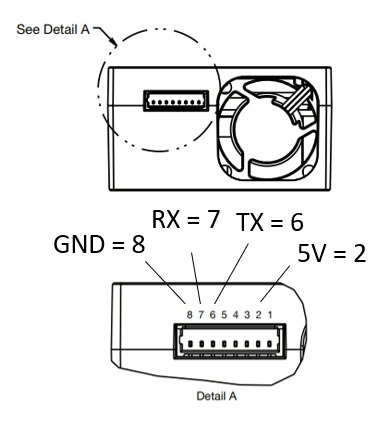
\includegraphics[height=9cm]{Images/HPMA115S0.png}
		\caption[HPMA115S0]{Pins required for use of the Honeywell \texttt{HPMA115S0} particulate sensor.
\texttt{TX} on the sensor should be connected wtih \texttt{RX} on the microcontroller and \texttt{RX} on the sensor should be connected with \texttt{TX} on the microcontroller.}
		\labfig{Honeywell}
	\end{center}
\end{marginfigure}

Air quality sensors operate by drawing a sample of air through a sensing device.
Measurement procedures depend on the physical characteristics of the pollutant of interest, but in general, most air quality sensors operate either by evaluating the light transmission properties of the sample or by measuring the electrochemical properties of an object in contact with the air.
The air sample must be drawn into the sampling area, usually using a fan or by allowing air to diffuse across a permeable barrier.
The procedures often involve steps such as enabling a fan or pre-heating the sampling chamber.
They sometimes require the user to change settings and/or trigger automatic calibration processes, so air quality sensors often include provisions for two-way \uart -based communication.

\begin{marginfigure}
	\begin{center}
		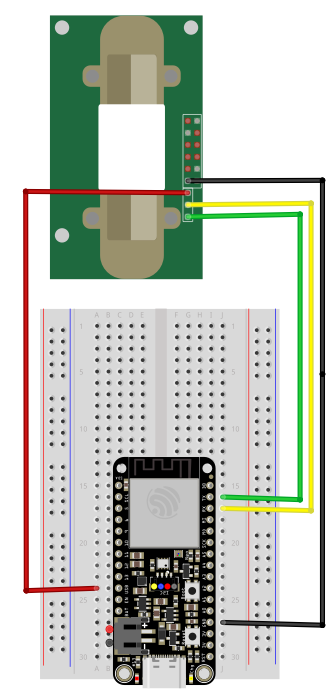
\includegraphics[height=10cm]{Images/mh-z14.png}
		\caption[MHZ14]{Circuit layout for \texttt{MH-Z14} carbon dioxide sensor. Note that some versions have slightly different pinout geometries, so if the geometry is not consistent with your sensor, use the following pins for making connections:  \texttt{Pin 19: TX}, \texttt{Pin 18: RX}, \texttt{Pin 17: Vin}, \texttt{Pin 16: GND}}
		\labfig{mh-z14}
	\end{center}
\end{marginfigure}

\begin{marginfigure}
	\begin{center}
		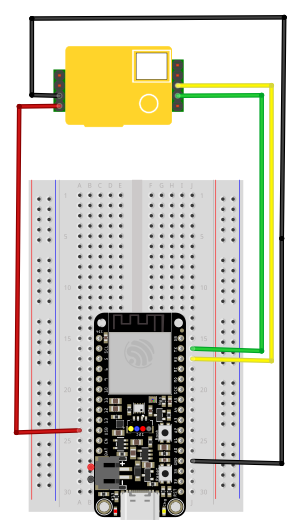
\includegraphics[height=10cm]{Images/mh-z19.png}
		\caption[MHZ19]{Circuit layout for \texttt{MH-Z19} carbon dioxide sensor.}
		\labfig{mh-z19}
	\end{center}
\end{marginfigure}

Operation is demonstrated here using either a Honeywell \texttt{HPMA115S0} particulate sensor or the Winson \texttt{MH-Z14/Z19} line of carbon dioxide sensors.
Both types of sensor evaluate the transmission of light within the sensor housing--for the particulate sensor, particulate concentration is correlated to scattering of light from a laser, and for the CO\textsubscript{2} sensors, concentration is estimated based on attenuation of a near-infrared light source as it passes through the air in the sensor cavity. Particulate results are reported in terms of the concentration of particles under 10 microns (PM10) or 2.5 microns (PM2.5), and CO\textsubscript{2} concentration is reported in terms of parts per million.

Pin diagrams and codes required to control \uart-based sensors are normally found in the datasheet for the sensor. Example datasheets are available online for both \htmladdnormallink{Honeywell HPMA particulate sensors}{https://sensing.honeywell.com/honeywell-sensing-hpm-series-particle-sensors-datasheet-32322550-e-en.pdf}, and the  \htmladdnormallink{MH-Z CO\textsubscript{2}}{https://sensing.honeywell.com/honeywell-sensing-hpm-series-particle-sensors-datasheet-32322550-e-en.pdf} sensors.
For the Honeywell sensor, the 5th page of the datasheet gives a specific sequence of bytes that we can send to the sensor to make it respond in a desired way.
Similar instructions are provided on pages 7 and 8 of the datsheet for the \texttt{MH-Z} sensors.  The datasheets also include sections describing where the necessary output pins (e.g., \texttt{TX}, \texttt{RX}, etc.) are located on sensors.
The necessary connections are shown in \reffig{Honeywell},  \reffig{mh-z14} and \reffig{mh-z19}. Note that while the \texttt{MH-Z14} and \texttt{MH-Z19} may look rather different, the same code can be used to control either sensor.

For any \uart -based sensor, the basic code initiation steps are the same.
To communicate over the \texttt{TX} and \texttt{RX} pins we’ve hooked up, we first have to define them.  
For this, first import the required libraries:
\begin{lstlisting}[language=Python]
import machine
import time
from machine import Pin
\end{lstlisting}

Note that while the time library is not strictly necessary for \uart communication, it can be important to provide delays while we wait for a sensor to respond, so it is helpful to import it now.
Then define a serial object we can manipulate on the desired microcontroller pins. For the \texttt{ESP32-S2}, the pins labeled \texttt{RX} and \texttt{TX} on the board are pins 38 and 39, respectively.
However, for most \texttt{ESP32} boards, \uart can be defined on any available GPIO pins.
 
\begin{lstlisting}[language=Python]
ser = machine.UART(1,baudrate=9600, rx=38, tx=39)
ser.init(9600, bits=8, parity=None, stop=1)
\end{lstlisting}

In the above, we also had to specify which \uart device from the microcontroller to use (device 1 here), as well as the communication rate (9600 bits per second), the number of bits in a packet (8), whether an error-checking mechanism known as \emph{parity} bits will be used, and how the end or \emph{stop} of a data packet is defined.
The settings must be consistent with whatever is specified in the sensor's datasheet.
However, with the possible excpetion of the relatively low baud rate, the settings shown here are quite commonly used in a large number of sensors.

\subsubsection{Communicating with Honeywell \texttt{HPMA115S0} particulate sensor over \uart}

After \uart has been initialized, we are ready to communicate with the device.
In the case of the Honeywell \texttt{HPMA115S0} sensor, the four bytes “0x68”, “0x01”, “0x04” and “0x93” (these are represented here as hexadecimal numbers—in Python, we have to represent them as “\textbackslash x68”, “\textbackslash x01”, “\textbackslash x04”, and “\textbackslash x93”), represent the command to read a measurement.
Once this is received by the sensor, it will send several bytes in response.
According to the datasheet, the first returned byte  is “0x40” (aka the “@” symbol), the second is “0x05”, the third is “0x04”, the next two bytes represent the PM2.5 measurement, and the next two bytes represent the PM10 measurement.
Then a final byte is sent finishing the transmission.
There are other commands that turn off the fan on the sensor and that turn off the “auto send” mode, which by default just keeps sending data about once a second even if we don’t request it (making interpreting the bytes in the serial data stream really difficult).

The default state of the sensor is to regularly stream data to the \uart.
We can read whatever it has sent to the microcontroller using \Micropython's readline() function: 

\begin{lstlisting}[language=Python]
ser.readline()
\end{lstlisting}

For the \texttt{HPMA} sensor, if you type this soon after the sensor was powered up, you’ll probably see uninterprable characters on your screen.
These represent the bytes that have been automatically sent by sensor to the microcontroller since the \uart was initialized.
The readline function just reads these bytes and prints them to the screen. It also has the effect of clearing the buffer, so if you do it again by typing

\begin{lstlisting}[language=Python]
ser.readline()
\end{lstlisting}

you may once again have one or two lines of characters, depending on how much time you waited and on whether the device is in autosend mode.

\paragraph{Turning off auto send}
The most helpful command at this point would be to tell the sensor to stop sending data to the microcontroller so frequently and filling up the \uart buffer.
We can do this by looking up this command in the datasheet, storing the code as a variable, then sending the variable to the sensor as follows:

\begin{lstlisting}[language=Python]
code = b"\x68\x01\x20\x77"
ser.readline()
ser.write(code)
time.sleep(1)
response = ser.readline()
print("command sent, acknowledgement is:")
print(response)
ser.readline()   #should be blank now that auto response is off
ser.readline()
\end{lstlisting}

In the first line of the above snippet, the “b” after the equal sign tells \Micropython we’re sending bytes, not \texttt{ASCII} text.
We must then enter the bytes using hexadecimal format.  We then do a readline() to clear the buffer so that we’re ready for whatever response the sensor gives.
The ser.write() function is what actually writes the four byte code to the sensor.
Next we wait for a second to give the sensor time to respond, then read the response into a variable called “response”.
We then print the response.  Finally, we test to make sure that we’re no longer getting data from the sensor every few seconds using a few more calls to the readline() function.

\paragraph{Controlling the fan}
If we were making measurements only every few minutes, we wouldn’t need the fan to be running the entire time, potentially filling our sensor with dust.  We can turn it off as follows:

\begin{lstlisting}[language=Python]
#turn reading off -- confirm that this stopped fan
stopcode= b"\x68\x01\x02\x95"
ser.readline()
ser.write(stopcode)
time.sleep(0.5)
response = ser.readline()
print("command sent, acknowledgement is:")
print(response)
\end{lstlisting}

If this worked, the fan should have stoped, and we should have received and printed the appropriate response from the sensor.
To turn it back on so that we are ready to make a reading, do the following:

\begin{lstlisting}[language=Python]
#turn reading on -- confirm that this started fan
startcode = b"\x68\x01\x01\x96"
ser.readline()
ser.write(startcode)
time.sleep(0.5)
response = ser.readline()
print("acknowledgement is:")
print(response)

\end{lstlisting}

The fan should start after the above snippet is sent.

\paragraph{Taking a sensor reading}
To actually take a reading, we use yet another code, as illustrated in the following snippet.

\begin{lstlisting}[language=Python]
#read particle measuring results -- 68 01 04 93
readcode = b"\x68\x01\x04\x93"
ser.readline()
ser.write(readcode)
time.sleep(1)
response = ser.readline()
PM25 = response[3]*256+response[4]
print("PM2.5 = ");
print(PM25)
PM10 = response[5]*256+response[6]
print("PM10 = ");
print(PM10)
\end{lstlisting}

Here, we define the code, clear the \uart buffer, send the code, wait for a response, read the response, and then convert the two appropriate bytes into the correct decimal value for the PM2.5 reading.
Note that we can refer to the fourth byte in the response by typing response[3] at the \texttt{REPL}.
The fifth byte is response[4].  When we multiply the bytes by a 256, Python knows that we are talking about multiplying the decimal equivalent by 256.
Then we simply print the results and do the same thing for the bytes associated with the PM10 reading.

\paragraph{Main loop}
Once we confirm we can get readings, we are ready to incorporate the code into a loop that takes the readings regularly and prints them to the screen.

\begin{lstlisting}[language=Python]
while True:
	readcode = b"\x68\x01\x04\x93"
	written = ser.write(readcode) 
	time.sleep(6)  #data sheet says response time is under 6 seconds
	response = ser.readline()
	print(response)
	if response[0] == 64 and len(response)==8:
		PM25 = response[3]*256+response[4]
		PM10 = response[5]*256+response[6]
		print(f"PM2.5 = {PM25}; PM10 = {PM10}")
	else:
		time.sleep(10)
		response = ser.readline()

\end{lstlisting}

In the above, the code that tells the sensor to take a reading, wait six seconds (the time the datasheet says is needed for a reading), read the response, then print it (in hexadecimal format).
There is always a chance that digital communication will not have been complete, so it's worth checking to be sure.
In this case, we look to see if the first character in the response is what we expect (so character “@” or decimal 64) and if we got the entire 8 bytes of the response (which we check using the “len” function).
If things look OK, we convert the appropriate bytes in the response to integer numbers and store these in the PM25 and PM10 variables.
The “print” command then prints these out, using a special way of formatting text that inserts the numerical value stored in the variable whereever Python sees the “\%s” symbol.
If we did not get a good response from the sensor, we wait 10 seconds before trying again.

\subsubsection{Communicating with Winson MH-Z14/19 carbon dioxide sensor over \uart}

Communication with the \texttt{MH-Z14} or \texttt{MH-Z19} sensors is similar to that with the \texttt{HPMA115S0 sensor}, but the sensor capabilities and the codes used to control it are quite different.
In the case of this sensor, only two main commands are likely to be needed by most users.
These are commands for taking a reading and for calibrating the sensor.
The datasheet suggests calibrating the sensor \emph{only} when it's been sitting in clean outdoor air likely to be at global ambient CO\textsubscript{2} concentration, so the calibration command should not be run unless that can be assured.
Additional detail regarding calibration is provided in the datasheet.

The following code defines the sequences of binary data that would either calibrate the sensor or perform a reading, respectively.
\begin{lstlisting}[language=Python]
#define codes
code_read = b"\xFF\x01\x86\x00\x00\x00\x00\x00\x79"
code_calibrate = b"\xFF\x01\x87\x00\x00\x00\x00\x00\x78"
\end{lstlisting}

If desired, the calibration can be performed simply by writing the calibtration code:
\begin{lstlisting}[language=Python]
#if calibration is desired, execute the following after sensor has been sitting in outdoor air for 20 minutes
ser.write(code_calibrate)
\end{lstlisting}

A reading can be taken, converted to the appropriate integer, and printed as follows:

\begin{lstlisting}[language=Python]
#take a reading
ser.readline()
#assign result to a variable so it won't print to screen
written = ser.write(code_read) 
time.sleep(1)
response = ser.readline()
print("acknowledgement is:")
print(response)
co2 = 256*response[2]+response[3]
print(f"CO2 = {co2}")
\end{lstlisting}

The readings can also be formatted and printed to the screen at regular intervals using the following code:

\begin{lstlisting}[language=Python]
#enter read loop
while True:
    ser.readline()
   #assign result to a variable so it won't print to screen
    written = ser.write(code_read) 
    time.sleep(5)
    try:
        response = ser.readline()
        co2 = 256*response[2]+response[3]
        print(f"CO2 = {co2}")
    except:
        pass
\end{lstlisting}

\newpage



\section{\spi sensors}
\labsec{spi_sensors}
\subsection{Background}
\spi is a ``4 wire'' protocol (in addition to \texttt{Vin} and \texttt{GND}).
However, three of these can be shared by multiple devices on the same \spi bus (the fourth must be unique to each device), so in some applications it is helpfully compact.
Technical details about \spi are at \htmladdnormallink{WikiPedia}{https://en.wikipedia.org/wiki/Serial\_Peripheral\_Interface\_Bus} and many other sources on the Internet.
One of the most useful explanations of the \spi protocol, in relation to \i2c and \uart, is provided by \htmladdnormallink{Sparkfun}{https://learn.sparkfun.com/tutorials/serial-peripheral-interface-spi/all}.

A single \spi bus can support multiple devices, each of which can transmit and receive data individually.
The focal device is specified by a ``chip select'' signal (over that 4th wire which is unique to each device).
This means there are no addressing conflicts, as can occur with \i2c.
Maximum data rates are higher for \spi than for \i2c or \uart devices.
Some digital sensors have both \spi and \i2c interfaces, so they can be used with either protocol.

As with \i2c, most microcontrollers have a built-in hardware \spi bus.
However, it is also often possible to ``bit-bang'' a software \spi bus, if the hardware \texttt{GPIO}s are not available.

%\sidenote[][*-12]{
	\begin{kaobox}[frametitle=Name that pin!]
		If there is a difficulty about the \spi interface, it is the variability in names for some of the \texttt{GPIO} connections.
		An \spi bus has one controlling device (almost always the  microcontroller), which sets the clock rate and determines which device is transmitting and receiving data at a given time.
		Originally, the connectors over which data are transmitted were called \texttt{MOSI} and \texttt{MISO}.
		That stood for ``Master Out, Slave In'' and ``Master In, Slave Out''.
		Because many users (the authors among them) \htmladdnormallink{found this nomenclature offensive}{https://www.oshwa.org/a-resolution-to-redefine-spi-signal-names}, a number of other names have come into use.

		In the \htmladdnormallink{Sparkfun}{https://learn.sparkfun.com/tutorials/serial-peripheral-interface-spi/all} tutorial, the pins are labeled \texttt{COPI} and \texttt{CIPO}, for ``Controller Out, Peripheral In'' and ``Controller In, Peripheral Out''.
		This more benignly preserves a property of the original labeling, that labels on all devices are consistent.

		Because it is rare for any device other than the microcontroller to act as the controller, the names in datasheets and labels on components have in many cases been shortened.
		For example, on the \esp8266 Feather, the \gpios connected to the hardware \spi bus are labeled \texttt{MO} (``Microcontroller Out'') and \texttt{MI} (``Microcontroller In'') without reference to the device.
		On many recent \spi devices, the corresponding labels are \texttt{DO} (``Device Out'') and \texttt{DI} (``Device In''), without reference to the controller.

		This can be slightly confusing, because labels are different on the microcontroller and peripheral devices.
	  However, you can keep it clear by keeping in mind that, like in \uart devices, data that go \underline{out} of one device go \underline{into} another.
	  As this implies, the \texttt{MO} \gpio is connected to the \texttt{DI} device pin, and the \texttt{MI} \gpio is connected to the \texttt{DO} device pin.
	\end{kaobox}
%}


\subsection{Connecting a microSD card through an \spi interface}
The addition of removable storage like a microSD card can hugely increase the capabilities of a microcontroller-based environmental sensor.
One reason for that is capacity: Onboard storage space on most microcontrollers amounts at most to 10s to 100s of megabytes (the \esp8266 is especially memory-constrained), while modern microSD cards with 10s to 100s of gigabytes are inexpensive and widely available.
Even voluminous data like very long time series can usually be recorded without much concern about space limitations on media of this size.

Another reason is accessibility: A microSD card can be programmed, inserted into an instrument, and extracted to retrieve data without ever needing to connect a cable to the microcontroller.
Those data can be read with almost any computer with a card reader or USB port.
A third reason is redundancy: Keeping duplicate copies of important codes and data on both a microcontroller's flash memory and a microSD card means that, if either fails, the information is not lost.

Microcontrollers that have a built-in microSD card reader, like the \texttt{ESP32CAM}, often have those readers hard-wired through internal connections to an \spi bus.
For those that don't, like the \esp8266, external microSD card readers utilizing the \spi interface are remarkably compact and inexpensive (we have been using \htmladdnormallink{these}{https://www.pjrc.com/store/sd_adaptor.html}, costing \$2, for many years).

\subsubsection{\howto Set up an external microSD card reader via \spi}

\begin{marginfigure}
	\begin{center}
		\htmladdnormallink{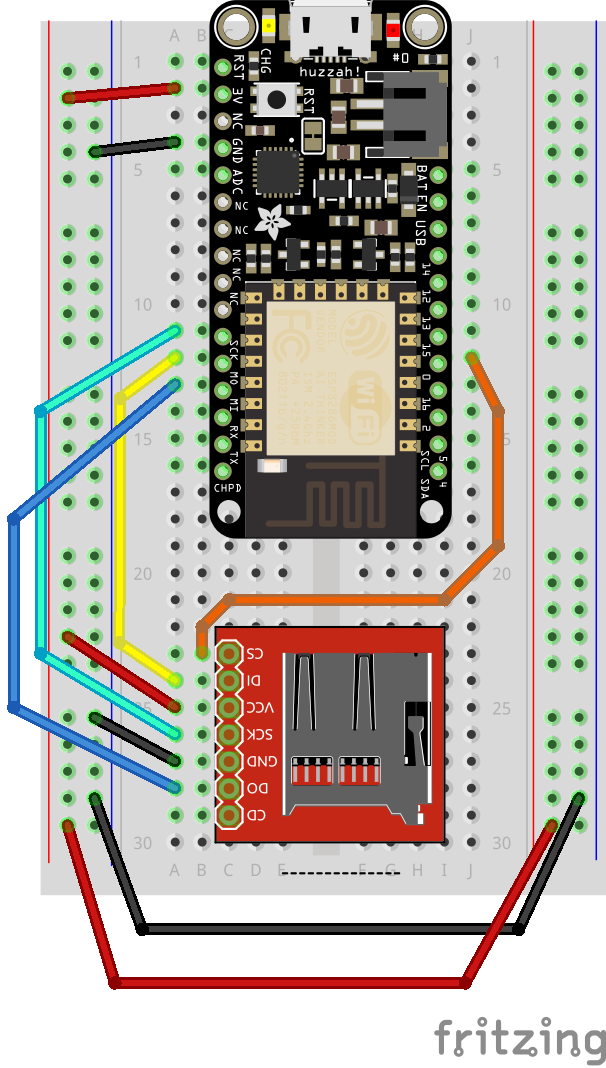
\includegraphics[width=\MFW]{Fritzing/feather_sdcard2_bb.png}}{https://github.com/publicsensors/IntroSensors/blob/digital/Fritzing/feather_sdcard2_bb.png}
		%\includegraphics[height=5cm]{Images/DS3231breadboard.jpg}
		\caption[microSD card on breadboard]{An example circuit with a microSD card reader connected to a microcontroller via the hardware \spi bus on an \esp8266 Feather.}
				\labfig{microSD}
	\end{center}
\end{marginfigure}

\begin{enumerate}
	\item \textbf{Connect pins or jumper wires to the GND, VCC, DO, DI, SCK and CS pins on the microSD card reader}.

	Note that there may be some variation in pin labeling.

	\item \textbf{Connect the GND and 3V pins on the ESP8266 to the GND and VCC pins on the microSD card reader}.

	The circuit layout for the \MCP9808 is shown in \reffig{microSD}.
	In this circuit, \texttt{GND} and \texttt{3V} are connected via the power rails, but any configuration that makes the apppropriate connections is OK.

	\item \textbf{Connect the \texttt{MI} pin on the ESP8266 to the \texttt{DO} pin on the microSD card reader. Similarly, connect \texttt{MO} to \texttt{DI} and \texttt{SCK} to \texttt{SCK}.}

	Note that, even though the \esp8266 Feather has \gpios labeled \texttt{MI}, \texttt{MO} and \texttt{SCK}, these are not actually separate pins.
	They are internally connected to \gpios on the other side of the microcontroller: the \texttt{MI} pin is really \gpio 12, \texttt{MO} is \gpio 13, and \texttt{SCK} is \gpio 14.

	\smallskip
	This means you can use \gpios 12, 13 and 14 to conect to the hrdware \spi bus, if they make your circuit layout more convenient.

	\smallskip
	On the other hand, \gpios 12, 13 and 14 are not available when using the hardware \spi bus, even if there is nothing directly connected to them.

	\item \textbf{Connect \gpio 15 on the ESP8266 to the \texttt{CS} pin on the microSD card reader.}

	This is the ``4th wire'', telling the reader when it is the device being addressed.
	It is fine to use another available \gpio, but make sure to modify the code below appropriately.

	\item \textbf{Download the driver for the SD card reader, \htmladdnormallink{sdcard.py}{https://raw.githubusercontent.com/publicsensors/IntroSensors/digital/Codes/sdcard.py}.}

	Save it into a \texttt{Codes} directory on your computer.

	\item \textbf{Copy } \lstinline{sdcard.py} \textbf{onto your microcontroller, using \thonny, \texttt{WebREPL} or \mpfshell (see the methods from \refch{connect} if you have questions).}

	This driver for \spi microSD card readers is part of the standard \Micropython library.
	However, it is omitted from most versions of firmware for the \esp8266, to save space.
	So usually you need to provide it on \esp8266 and some other smaller microcontrollers.

	\item \textbf{Format a FAT32 microSD card}

	It is possible to format a microSD ard using the reader itself, but we suggest you use your computer.
	For one thing, this makes it easy to see whether there are files you care about already on the card -- these will be irretrievably erased when the card is reformatted.
	It is also helpful in debugging, because it separates the formatting step from getting basic file writing and reading to work in a new circuit.

	\item \textbf{Copy a sample code onto the microSD card}

	This simple code will serve as an example and test of reading and executing code off the microSD card, rather than the microcontroller's built-in flash memory:
	\lstinputlisting[language=Python,label=sd_hello,caption={\htmladdnormallink{\texttt{sd\textunderscore hello.py}}{https://github.com/publicsensors/IntroSensors/blob/main/Codes/sd_hello.py}: An example to test reading and executing code from an SD card.}]{Codes/sd_hello.py}

	\item \textbf{Insert the FAT32 formatted microSD card into the reader}

	\item \textbf{Initialize the microSD card object}

	Type in and execute the following lines, one by one, into your microcontroller's \texttt{REPL}:
\begin{lstlisting}[language=Python]
import machine, sdcard, os, sys
sd = sdcard.SDCard(machine.SPI(1), machine.Pin(15))
os.mount(sd, '/sd')
os.listdir('/')
\end{lstlisting}
  With these commands, you performed three necessary steps.
  First, you imported modules that you will need to access the microSD card.
  Next, you created an sdcard object, named ``\texttt{sd}''.
  Then, you ``mounted'' the \texttt{sd} object into the filesystem as a subdirectory, under \texttt{/sd}.

  \smallskip
	The last command simply lists the files in the main directory on the microcontroller.
  The output should be a list of files, something like
\begin{lstlisting}[language=Python]
 ['sd', 'boot.py', 'main.py']
\end{lstlisting}
 The list should include whichever Python codes and other files or directories you have on your microcontroller.
 The main point now, however, is that you should see the \texttt{sd} entry appear.
 This shows that the microSD card is now visible to the filesystem.

	\item \textbf{Add the SD card to the filesystem path}

	The filesystem on your microcontroller has a list of locations in which it looks for codes to import.
	To see this list, execute the command
\begin{lstlisting}[language=Python]
sys.path
\end{lstlisting}
 The output will be something like
\begin{lstlisting}[language=Python]
['', '/lib', '/']
\end{lstlisting}
 This shows that the current locations in the filesystem in which the microcontroller looks for modules to import are the current working directory (''), the root of the filesystem ('/'), and a library subdirectory ()'/lib').
 Note that these do not include the microSD card, meaning codes on the card are not visible for import.

 \smallskip
 Now, execute:
 \begin{lstlisting}[language=Python]
sys.path.append("/sd")
sys.path
\end{lstlisting}
 The first of these adds "/sd" to the path list.
 The second prints out the augmented list, which should now include the microSD card:
\begin{lstlisting}[language=Python]
['', '/lib', '/', '/sd']
\end{lstlisting}
This shows that the microcontroller will now also look in the "/sd" subdirectory for modules to import.

	\item \textbf{Import the \texttt{sd\textunderscore hello.py} module from the microSD card}:
\begin{lstlisting}[language=Python]
import sd_hello
\end{lstlisting}
 The module should now load, giving the output:
\begin{lstlisting}[language=Python]
hello sdcard!
\end{lstlisting}

 If you got this output, you have successfully added a microSD card to your microcontoller's filesystem, and run code from it.
\end{enumerate}
\loadMilestone{mlst:05c} % load milestone with tags id: mlst:05c

% \subsection{\color{gray} SPI control of a TFT display panel \color{black}}


%
% \vspace{10cm}
%
%
% \section{Construction, calibration and use of a colorometric pH sensor}
% \labsec{pH_sensor}
% Placeholder for pH sensor section.
